% This is "sig-alternate.tex" V2.1 April 2013
% This file should be compiled with V2.5 of "sig-alternate.cls" May 2012
%
% This example file demonstrates the use of the 'sig-alternate.cls'
% V2.5 LaTeX2e document class file. It is for those submitting
% articles to ACM Conference Proceedings WHO DO NOT WISH TO
% STRICTLY ADHERE TO THE SIGS (PUBS-BOARD-ENDORSED) STYLE.
% The 'sig-alternate.cls' file will produce a similar-looking,
% albeit, 'tighter' paper resulting in, invariably, fewer pages.
%
% ----------------------------------------------------------------------------------------------------------------
% This .tex file (and associated .cls V2.5) produces:
%       1) The Permission Statement
%       2) The Conference (location) Info information
%       3) The Copyright Line with ACM data
%       4) NO page numbers
%
% as against the acm_proc_article-sp.cls file which
% DOES NOT produce 1) thru' 3) above.
%
% Using 'sig-alternate.cls' you have control, however, from within
% the source .tex file, over both the CopyrightYear
% (defaulted to 200X) and the ACM Copyright Data
% (defaulted to X-XXXXX-XX-X/XX/XX).
% e.g.
% \CopyrightYear{2007} will cause 2007 to appear in the copyright line.
% \crdata{0-12345-67-8/90/12} will cause 0-12345-67-8/90/12 to appear in the copyright line.
%
% ---------------------------------------------------------------------------------------------------------------
% This .tex source is an example which *does* use
% the .bib file (from which the .bbl file % is produced).
% REMEMBER HOWEVER: After having produced the .bbl file,
% and prior to final submission, you *NEED* to 'insert'
% your .bbl file into your source .tex file so as to provide
% ONE 'self-contained' source file.
%
% ================= IF YOU HAVE QUESTIONS =======================
% Questions regarding the SIGS styles, SIGS policies and
% procedures, Conferences etc. should be sent to
% Adrienne Griscti (griscti@acm.org)
%
% Technical questions _only_ to
% Gerald Murray (murray@hq.acm.org)
% ===============================================================
%
% For tracking purposes - this is V2.0 - May 2012

\documentclass{sig-alternate-05-2015}

%\usepackage{url}

%!TEX root = main.tex

\usepackage{fancybox}
\usepackage{graphicx}
\graphicspath{{figures/}}
\DeclareGraphicsExtensions{.pdf,.jpeg,.png}
\usepackage{amsmath}
\usepackage{subfigure}
\usepackage{caption}
\usepackage{fancyvrb}
\usepackage{color}
\usepackage{algorithmic}
\usepackage{array}
\usepackage{hyperref}
\usepackage{mdwmath}
\usepackage{mdwtab}
\usepackage{booktabs}
\usepackage{listings}
\usepackage{eqparbox}
\usepackage{stfloats}
\usepackage{url}
\usepackage{comment}
\usepackage{framed}
%\usepackage{pdfsync}
\usepackage{ifthen}
\usepackage{balance}
% call this with optional  [turnoff] to turn off notes and todos
%\usepackage[turnoff]{notes}
\usepackage[turnon]{notes}
\usepackage{multirow}
\usepackage{xspace}
\usepackage{listings}
\usepackage[noabbrev]{cleveref}
%\usepackage[table]{xcolor}



\setlength{\belowcaptionskip}{-11pt}

\renewcommand{\baselinestretch}{0.99}

\newcommand{\rom}[1]{\uppercase\expandafter{\romannumeral #1\relax}}

\newcommand{\cf}{\hbox{\emph{cf.}}\xspace}
\newcommand{\deletia}{\ldots [deletia] \ldots}
\newcommand{\etal}{\hbox{\emph{et al.}}\xspace}
\newcommand{\eg}{\hbox{\emph{e.g.,}}\xspace}
\newcommand{\ie}{\hbox{\emph{i.e.}}\xspace}
\newcommand{\st}{\hbox{\emph{s.t.}}\xspace}
\newcommand{\wrt}{\hbox{\emph{w.r.t.}}\xspace}
\newcommand{\viz}{\hbox{\emph{viz.}}\xspace}
\newcommand{\vs}{\hbox{\emph{v.s.}}\xspace}
\newcommand{\etc}{\hbox{\emph{etc.}}\xspace}

\newcommand{\cache}{\hbox{{\$gram }}\xspace}

\newtheorem{theorem}{Theorem}[section]
\newcommand{\defref}[1]{Definition~\ref{#1}}
\newtheorem{definition}[theorem]{Definition}

\newcommand{\varname}[1]{{\small\texttt{#1}}\xspace}
%\newcommand{\tom}[1]{{\color{red} Tom: #1}\xspace}
\newcommand{\ch}[1]{{\color{black} #1}\xspace}
%\newfloatcommand{capbtabbox}{table}[][\FBwidth]

\newcommand{\DP}{DP\xspace}


\newcommand{\nbf}{\hbox{${\cal N}\hspace{-0.01in}{\cal B}\hspace{-0.01in}{\cal F}$}\xspace}
\newcommand{\sta}{\hbox{${\cal S}\hspace{-0.01in}{\cal B}\hspace{-0.01in}{\cal F}$}\xspace}
\newcommand{\dpm}{\hbox{${\cal D}\hspace{-0.01in}{\cal P}$}\xspace}
%\newcommand{\ngm}{\hbox{${\cal \$}\hspace{-0.01in}{\cal G}\hspace{-0.01in}{\cal R}\hspace{-0.01in}{\cal A}\hspace{-0.01in}{\cal M}$}\xspace}






\newcommand{\bray}[1]{{\scriptsize \todo{Bray:  {\color{red} #1}}}}


\newcommand{\tableshrink}[1]{\vspace{-0.25in}}



\definecolor{gray50}{gray}{.5}
\definecolor{gray40}{gray}{.6}
\definecolor{gray30}{gray}{.7}
\definecolor{gray20}{gray}{.8}
\definecolor{gray10}{gray}{.9}
\definecolor{gray05}{gray}{.95}

\newlength\Linewidth
\def\findlength{\setlength\Linewidth\linewidth
\addtolength\Linewidth{-4\fboxrule}
\addtolength\Linewidth{-3\fboxsep}
}
\newenvironment{examplebox}{\par\begingroup
   \setlength{\fboxsep}{5pt}\findlength
   \setbox0=\vbox\bgroup\noindent
   \hsize=0.95\linewidth
   \begin{minipage}{0.95\linewidth}\normalsize}
    {\end{minipage}\egroup
%    \vspace{6pt}
    \textcolor{gray20}{\fboxsep1.5pt\fbox
     {\fboxsep5pt\colorbox{gray05}{\normalcolor\box0}}}
%    \endgroup\par\addvspace{6pt minus 3pt}\noindent
    \endgroup\par\noindent
    \normalcolor\ignorespacesafterend}
\let\Examplebox\examplebox
\let\endExamplebox\endexamplebox

%-------------------------------------------------------------------------------------------
% Research Questions and Results
%
\newcounter{RQCounter}
\newcounter{RQACounter}

 %Pass in label for rq, then rq
%

\newcommand{\RQ}[2]{%
\refstepcounter{RQCounter} \label{#1}
 \begin{center}	
  \begin{examplebox}
   \textbf{RQ\arabic{RQCounter}.}~#2
  \end{examplebox}	 
 \end{center}
}

\newcommand{\RQA}[2]{%
\refstepcounter{RQACounter} \label{#1}
\vspace{0.1in} \noindent\textbf{RQ\arabic{RQACounter}.~#2 \vspace{0.05in}}

}

\newcommand{\RQBoxed}[2]{%
\refstepcounter{RQCounter} \label{#1}
\begin{framed}%
\filbreak
\vspace{0.001in}
	%\noindent\textbf{Research Question \arabic{RQCounter}: }%
	\noindent\textbf{RQ\arabic{RQCounter}: }%
#2\end{framed}
}


% Pass in label for associated research question
%
\newcommand{\RS}[2]{%
\begin{framed}%
\filbreak
	%\noindent
\textbf{Result {\ref{#1}}:~}{\emph {#2}}%
\end{framed}
}

\definecolor{javared}{rgb}{0.6,0,0} % for strings
\definecolor{javagreen}{rgb}{0.25,0.5,0.35} % comments
\definecolor{javapurple}{rgb}{0.5,0,0.35} % keywords
\definecolor{javadocblue}{rgb}{0.25,0.35,0.75} % javadoc


\lstdefinestyle{customc}{
  belowcaptionskip=\baselineskip,
  breaklines=true,
 % frame=L,
  xleftmargin=\parindent,
  language=java,
  showstringspaces=false,
  basicstyle=\scriptsize\ttfamily,
  keywordstyle=\bfseries\color{javapurple},
  commentstyle=\itshape\blue,
%  identifierstyle=\blue,
%  stringstyle=\color{javared},
  belowskip=-10pt,
  aboveskip=-5pt
%  numbers=left,
 % numberstyle=\tiny\,
}

\lstset{escapechar=@,style=customc}


\newcommand\at{@}
\newcommand\lb{[}
\newcommand\rb{]}
\newcommand\Red[1]{\textcolor[rgb]{1.00,0.00,0.00}{\textbf{#1}}}
\newcommand\red[1]{\textcolor[rgb]{1.00,0.00,0.00}{#1}}
\newcommand\grayline[1]{\textcolor[rgb]{0.4,0.4,0.4}{{#1}}}
\newcommand\gray[1]{\colorbox[rgb]{0.8,0.8,0.8}{{#1}}}
\newcommand\brown[1]{\textcolor[rgb]{0.55,0.27,0.07}{#1}}
\newcommand\orange[1]{\textcolor[rgb]{1.00,0.55,0.30}{\textbf{#1}}}
%\newcommand\green[1]{\textcolor[rgb]{0.42,0.56,0.14}{#1}}
\newcommand\lime[1]{\textcolor[rgb]{0.13,0.55,0.13}{{#1}}}
\newcommand\blue[1]{\textcolor[rgb]{0.00,0.00,1.00}{{#1}}}
\newcommand\ColorLine[1]{\textcolor[rgb]{0.00,0.00,1.00}{{#1}}}
\newcommand\javagreen[1]{\textcolor[rgb]{0.25,0.5,0.35}{{#1}}}
\newcommand\javadocblue[1]{\textcolor[rgb]{0.25,0.35,0.75}{{#1}}}
\newcommand\dkgreen[1]{\textcolor[rgb]{0.0,0.6,0}{\textbf{#1}}}
\newcommand\green[1]{\textcolor[rgb]{0.0,0.6,0}{#1}}
\newcommand\mauve[1]{\textcolor[rgb]{0.58,0.0,0.82}{{#1}}}
\newcommand\yellow[1]{\textcolor[rgb]{1,0.9,0.5}{{\bf #1}}}
\newcommand\lblue[1]{\colorbox[rgb]{0.87,1,1}{{#1}}}

\newcommand\PYbg[1]{\textcolor[rgb]{0.00,0.50,0.00}{\textbf{#1}}}
\newcommand\PYbf[1]{\textcolor[rgb]{0.73,0.40,0.53}{\textbf{#1}}}
\newcommand\PYbe[1]{\textcolor[rgb]{0.40,0.40,0.40}{#1}}
\newcommand\PYbd[1]{\textcolor[rgb]{0.73,0.13,0.13}{#1}}
\newcommand\PYbc[1]{\textcolor[rgb]{0.00,0.50,0.00}{\textbf{#1}}}
\newcommand\PYbb[1]{\textcolor[rgb]{0.40,0.40,0.40}{#1}}
\newcommand\PYba[1]{\textcolor[rgb]{0.00,0.00,0.50}{\textbf{#1}}}
\newcommand\PYaJ[1]{\textcolor[rgb]{0.73,0.13,0.13}{#1}}
\newcommand\PYaK[1]{\textcolor[rgb]{0.00,0.00,1.00}{\textbf{#1}}}
\newcommand\PYaH[1]{\fcolorbox[rgb]{1.00,0.00,0.00}{1,1,1}{#1}}
\newcommand\PYaI[1]{\textcolor[rgb]{0.69,0.00,0.25}{#1}}
\newcommand\PYaN[1]{\textcolor[rgb]{0.00,0.00,1.00}{\textbf{#1}}}
\newcommand\PYaO[1]{\textcolor[rgb]{0.00,0.00,0.50}{\textbf{#1}}}
\newcommand\PYaL[1]{\textcolor[rgb]{0.73,0.73,0.73}{#1}}
\newcommand\PYaM[1]{\textcolor[rgb]{0.74,0.48,0.00}{#1}}
\newcommand\PYaB[1]{\textcolor[rgb]{0.00,0.25,0.82}{#1}}
\newcommand\PYaC[1]{\textcolor[rgb]{0.67,0.13,1.00}{#1}}
\newcommand\PYaA[1]{\textcolor[rgb]{0.00,0.50,0.00}{#1}}
\newcommand\PYaF[1]{\textcolor[rgb]{1.00,0.00,0.00}{#1}}
\newcommand\PYaG[1]{\textcolor[rgb]{0.10,0.09,0.49}{#1}}
\newcommand\PYaD[1]{\textcolor[rgb]{0.25,0.50,0.50}{\textit{#1}}}
\newcommand\PYaE[1]{\textcolor[rgb]{0.63,0.00,0.00}{#1}}
\newcommand\PYaZ[1]{\textcolor[rgb]{0.00,0.50,0.00}{\textbf{#1}}}
\newcommand\PYaX[1]{\textcolor[rgb]{0.00,0.50,0.00}{#1}}
\newcommand\PYaY[1]{\textcolor[rgb]{0.73,0.13,0.13}{#1}}
\newcommand\PYaR[1]{\textcolor[rgb]{0.10,0.09,0.49}{#1}}
\newcommand\PYaS[1]{\textcolor[rgb]{0.25,0.50,0.50}{\textit{#1}}}
\newcommand\PYaP[1]{\textcolor[rgb]{0.49,0.56,0.16}{#1}}
\newcommand\PYaQ[1]{\textcolor[rgb]{0.40,0.40,0.40}{#1}}
\newcommand\PYaV[1]{\textcolor[rgb]{0.00,0.00,1.00}{\textbf{#1}}}
\newcommand\PYaW[1]{\textcolor[rgb]{0.73,0.13,0.13}{#1}}
\newcommand\PYaT[1]{\textcolor[rgb]{0.50,0.00,0.50}{\textbf{#1}}}
\newcommand\PYaU[1]{\textcolor[rgb]{0.82,0.25,0.23}{\textbf{#1}}}
\newcommand\PYaj[1]{\textcolor[rgb]{0.00,0.50,0.00}{#1}}
\newcommand\PYak[1]{\textcolor[rgb]{0.73,0.40,0.53}{#1}}
\newcommand\PYah[1]{\textcolor[rgb]{0.63,0.63,0.00}{#1}}
\newcommand\PYai[1]{\textcolor[rgb]{0.10,0.09,0.49}{#1}}
\newcommand\PYan[1]{\textcolor[rgb]{0.67,0.13,1.00}{\textbf{#1}}}
\newcommand\PYao[1]{\textcolor[rgb]{0.73,0.40,0.13}{\textbf{#1}}}
\newcommand\PYal[1]{\textcolor[rgb]{0.25,0.50,0.50}{\textit{#1}}}
\newcommand\PYam[1]{\textbf{#1}}
\newcommand\PYab[1]{\textit{#1}}
\newcommand\PYac[1]{\textcolor[rgb]{0.73,0.13,0.13}{#1}}
\newcommand\PYaa[1]{\textcolor[rgb]{0.50,0.50,0.50}{#1}}
\newcommand\PYaf[1]{\textcolor[rgb]{0.25,0.50,0.50}{\textit{#1}}}
\newcommand\PYag[1]{\textcolor[rgb]{0.40,0.40,0.40}{#1}}
\newcommand\PYad[1]{\textcolor[rgb]{0.73,0.13,0.13}{#1}}
\newcommand\PYae[1]{\textcolor[rgb]{0.40,0.40,0.40}{#1}}
\newcommand\PYaz[1]{\textcolor[rgb]{0.00,0.63,0.00}{#1}}
\newcommand\PYax[1]{\textcolor[rgb]{0.60,0.60,0.60}{\textbf{#1}}}
\newcommand\PYay[1]{\textcolor[rgb]{0.00,0.50,0.00}{\textbf{#1}}}
\newcommand\PYar[1]{\textcolor[rgb]{0.10,0.09,0.49}{#1}}
\newcommand\PYas[1]{\textcolor[rgb]{0.73,0.13,0.13}{\textit{#1}}}
\newcommand\PYap[1]{\textcolor[rgb]{0.00,0.50,0.00}{#1}}
\newcommand\PYaq[1]{\textcolor[rgb]{0.53,0.00,0.00}{#1}}
\newcommand\PYav[1]{\textcolor[rgb]{0.00,0.50,0.00}{\textbf{#1}}}
\newcommand\PYaw[1]{\textcolor[rgb]{0.40,0.40,0.40}{#1}}
\newcommand\PYat[1]{\textcolor[rgb]{0.10,0.09,0.49}{#1}}
\newcommand\PYau[1]{\textcolor[rgb]{0.40,0.40,0.40}{#1}}


\usepackage{multirow}


\begin{document}

% Copyright

%UNCOMMENT STUFF BEFORE DELIVERY
\setcopyright{acmcopyright}
%\setcopyright{acmlicensed}
%\setcopyright{rightsretained}
%\setcopyright{usgov}
%\setcopyright{usgovmixed}
%\setcopyright{cagov}
%\setcopyright{cagovmixed}


% DOI
\doi{}

% ISBN
\isbn{}

%Conference
\conferenceinfo{MSR '16}{May 14--15, 2016, Austin, TX, USA}

%\acmPrice{\$}

%
% --- Author Metadata here ---
\conferenceinfo{The 13th Working Conference on Mining Software Repositories}{'16 Austin, Texas USA}
%\CopyrightYear{2007} % Allows default copyright year (20XX) to be over-ridden - IF NEED BE.
%\crdata{0-12345-67-8/90/01}  % Allows default copyright data (0-89791-88-6/97/05) to be over-ridden - IF NEED BE.
% --- End of Author Metadata ---

\title{Ownership and Defects in Open-Source Software}
%\titlenote{(Produces the permission block, and copyright information). For use with SIG-ALTERNATE.CLS. Supported by ACM.}}
%\subtitle{<Subtitle?>}


%
% You need the command \numberofauthors to handle the 'placement
% and alignment' of the authors beneath the title.
%
% For aesthetic reasons, we recommend 'three authors at a time'
% i.e. three 'name/affiliation blocks' be placed beneath the title.
%
% NOTE: You are NOT restricted in how many 'rows' of
% "name/affiliations" may appear. We just ask that you restrict
% the number of 'columns' to three.
%
% Because of the available 'opening page real-estate'
% we ask you to refrain from putting more than six authors
% (two rows with three columns) beneath the article title.
% More than six makes the first-page appear very cluttered indeed.
%
% Use the \alignauthor commands to handle the names
% and affiliations for an 'aesthetic maximum' of six authors.
% Add names, affiliations, addresses for
% the seventh etc. author(s) as the argument for the
% \additionalauthors command.
% These 'additional authors' will be output/set for you
% without further effort on your part as the last section in
% the body of your article BEFORE References or any Appendices.

\numberofauthors{2} %  in this sample file, there are a *total*
% of EIGHT authors. SIX appear on the 'first-page' (for formatting
% reasons) and the remaining two appear in the \additionalauthors section.
%
\author{
% You can go ahead and credit any number of authors here,
% e.g. one 'row of three' or two rows (consisting of one row of three
% and a second row of one, two or three).
%
% The command \alignauthor (no curly braces needed) should
% precede each author name, affiliation/snail-mail address and
% e-mail address. Additionally, tag each line of
% affiliation/address with \affaddr, and tag the
% e-mail address with \email.
%
% 1st. author
\alignauthor
Eric Camellini\\
       \affaddr{Politecnico di Milano}\\
    %   \affaddr{1932 Wallamaloo Lane}\\
       \affaddr{Milan, Italy}\\
       \email{Eric.Camellini@gmail.com}
% 2nd. author
\alignauthor
Kaj Dreef\\
       \affaddr{Delft University of Technology}\\
    %   \affaddr{P.O. Box 1212}\\
       \affaddr{Delft, The Netherlands}\\
       \email{Kaj.Dreef@gmail.com}
}


\maketitle

\begin{abstract}
Code ownership measures the proportion of contribution of the developers to a source code artifact, in terms of code changes (e.g. number of commits). It can be used to describe the responsibility for a certain piece of software or the expertise of the developers with respect to it. Responsibility and expertise are important factors in the development process, and can affect software quality: for this reason a lot of studies focused on determining how to measure the ownership in order to include it in defect prediction models in an effective way. Bird et al~\cite{bird:original} and Greiler et al.~\cite{Greiler:replication} showed that ownership metrics are a good indicator for software quality in Microsoft software projects, while Foucault et al.~\cite{Foucault:oss} found contrasting results for what concerns open-source software projects. However, in our opinion these past studies compute the ownership without considering the software revisions that actually introduce defects. Furthermore, no study did an explicit analysis of the effect of the granularity chosen to consider the code changes (e.g. considering lines instead of commits).

In this paper we contribute to the past research in the following ways: (1) we build dataset, publicly available, that contains information about code changes and defects over the whole development history for five open-source software projects; (2) we describe and apply a novel technique to compute software metrics, using the above mentioned dataset, that can capture the state of the software right after the introduction of defective code; (3) we use this technique to empirically study the effect that ownership has on software quality for five open-source software projects, considering an exhaustive set of metrics in terms of granularity of code changes.

Using this approach and considering also a set of classic and effective code metrics we are able to classify defective files, using Random Forest, with an average out-of-bag error rate of 23\% and an average relative improvement of 22\% over a model that uses only the classic metrics. %Also line based metrics have on average a performance increase of 17\% in comparison to commit based metrics.
\end{abstract}


%
% The code below should be generated by the tool at
% http://dl.acm.org/ccs.cfm
% Please copy and paste the code instead of the example below.
%
\begin{CCSXML}
<ccs2012>
<concept>
<concept_id>10011007.10011074.10011099.10011102</concept_id>
<concept_desc>Software and its engineering~Software defect analysis</concept_desc>
<concept_significance>500</concept_significance>
</concept>
<concept>
<concept_id>10011007.10011074.10011134.10003559</concept_id>
<concept_desc>Software and its engineering~Open source model</concept_desc>
<concept_significance>300</concept_significance>
</concept>
<concept>
<concept_id>10002951.10003227.10003351</concept_id>
<concept_desc>Information systems~Data mining</concept_desc>
<concept_significance>100</concept_significance>
</concept>
</ccs2012>
\end{CCSXML}

\ccsdesc[500]{Software and its engineering~Software defect analysis}
\ccsdesc[300]{Software and its engineering~Open source model}
\ccsdesc[100]{Information systems~Data mining}


%
% End generated code
%

%
%  Use this command to print the description
%

\printccsdesc

% We no longer use \terms command
%\terms{Theory}

\keywords{Ownership; Software quality; Process metrics}



\section{Introduction}
\label{sec:introduction}
Software defects correction have a great impact on the economy: it costs tens of billions of dollars every year and the 50\% of developers programming time \cite{DefectsCost, DefectsCost2}. For this reason, in recent years, a wide number of studies focused on defining and comparing software metrics that can be useful to build models for \textit{defect prediction} \cite{bird:original, Rahman:blame, Greiler:replication, Rahman:2013, moser2008comparative, zimmermann2009cross-project}. A \textit{software metric} is a measure of a property of the software that can be related to the code (\textit{code metric}) or to its development process (\textit{process or change metric}). Previous studies also reported that process metrics are better-suited for prediction models \cite{moser2008comparative, Rahman:2013}. These past results showed that the developers behaviour has more impact on software quality than the characteristics of the software itself. \textit{Code ownership} metrics are process metrics, and can in general be defined as measurements of the proportion of contribution of the developers to a source code artifact over a certain period of time, in terms of code changes (e.g. number of commits) \cite{Greiler:replication}.

Previous studies reported contrasting results on the relation between software quality and ownership; this is probably due to the fact that ownership metrics are highly dependant on the process used to develop the software and on the organizational structure of the team. Bird et al.~\cite{bird:original} showed that there is a significant correlation between ownership and number of defects in Microsoft Windows projects, while accordingly to Foucault et al.~\cite{Foucault:oss} the same metrics do not result in the same kind of relationship when computed on open-source software (OSS) artifacts. Foucault et al.~\cite{Foucault:oss} also introduced the idea of computing ownership metrics on artifacts of different granularities (Java files and packages). Greiler et al.~\cite{Greiler:replication} applied the same principle on different Microsoft Products, and their results showed that it can be more significant to use ownership metrics to classify defective and non-defective artifacts rather than to try to infer the number of defects. 

%NOT NEEDED: 
%To obtain more generalizable results ownership metrics should be computed in a way that adapts to the structure of the project.

%Unfortunately, to our knowledge, a classification approach like the one described above has not yet been applied to Open-Source Software. Furthermore, none of the previous studies tried to compute the ownership metrics on the revision of the artifact where the defective code is introduced. In addition to that, all the previously cited works computed the ownership metrics considering as variable the commit count on the software artifacts, and tried to change the granularity of the artifacts themselves, but not the granularity of the considered variable (e.g. considering the amount of lines added and deleted in every commit instead of the commit count).

All the previous studies computed the metrics on a certain release of the software and then tried to find a correlation between these metrics and the number of defects introduced before that release. We think that the metrics should instead be computed on the software artifacts just after the commits that introduce a defect, to better capture the exact state of the code when it becomes defective. In addition to that, most of the previously cited works used the commit count to measure the contribution of the developers to the source code artifacts; none of them tried to compute the ownership metrics in a more fine-grained way (e.g. considering the amount lines of code added and deleted). Furthermore, to our knowledge, a classification approach like the one described in in the previous paragraph has not yet been applied to Open-Source Software.

%Our idea is that in order to build a defect prediction model the ownership metrics should be computed on the releases of software artifacts that succeed the introduction of defective code. 
%To determine when the defective code is introduced we use the concept of \textit{implicated code} as described by Rahman er al.~\cite{Rahman:blame} (also called \textit{fix-inducing} code~\cite{sliwerski2005changes}). 

In this work, we study the effect of code ownership on software quality by trying to classify defective source code files on different Open-Source software projects. We expand the cited previous work by: (1) computing ownership metrics on source files just after some defective code is introduced; (2) experimenting the effects of changing the granularity of the metrics; (3) applying a classification approach to distinguish defective and non-defective source files on Open-Source software projects.

To spot the introduction of defective code we use the concept of \textit{implicated code} as described by Rahman et al.~\cite{Rahman:blame} (also called \textit{fix-inducing} code~\cite{sliwerski2005changes}). 
We selected 5 OSS projects and, for each one of them, we: (1) create  a dataset that captures the history of its development in terms of developers contribution and implicated code introduction (2) use this dataset to create a second dataset that contains the ownership metrics computed for every version of every file, with different granularities (3) use these metrics, together with some classic defect prediction code metrics, to classify the defective file versions with the Random Forests~\cite{breiman2001random} and Logistic Regression techniques (4) measure how the ownership metrics improve the model that uses only the classic ones.

Our results show that ownership metrics are indicative for software defects, giving a significant improvement over a classification model built using only classic code metrics; this is particularly evident when using a more fine-grained, line-based, approach to compute the ownership, as we hypothesized.

We think that our approach can capture the characteristics of the defective code in a better way, leading to more generalizable outcomes.

Code and datasets created for this work are publicly available.\footnote{\url{github.com/kajdreef/IN4334-MSR}}


%!Tex root=../main.tex

\section{The problem}
\label{sec:prob}

The general problem that is targeted in this paper is that building software defect prediction models is a challenging activity, and one of its main difficulties is that it is highly project-dependant~\cite{zimmermann2009cross-project}.
In particular we address this problem for models built using \textit{code ownership} metrics. Code ownership is a measurement of the proportion of contribution of the developers to a source code artifact over a certain period of time, in terms of code changes (e.g. number of commits) \cite{Greiler:replication}. It describes whether the \textit{responsibility} for a certain software artifact is spread around many developers, or if there is a single person that can be considered its ``owner'';  it can also be interpreted as a measure of the \textit{expertise} of a developer with respect to the code artifact~\cite{bird:original}.

%past studies showed that, on Microsoft products, code artifacts without a clear responsible are more defect prone \cite{bird:original,  Greiler:replication}. In these studies ownership is also interpreted as a measure of the \textit{expertise} of a developer with respect to the code artifact.

This work addresses the more specific problem that currently it is difficult to generalize the effect of code ownership on software quality; previous studies show contrasting result when trying to correlate these two aspects~\cite{bird:original, Foucault:oss, Greiler:replication}. What makes the problem complicated is that code ownership highly depends on the organizational structure of the development team and on the developers behaviour.

\subsection{Existing solutions and limitations}
\label{sec:existing_solutions}
The main source of inspiration for us comes from Bird et
al.~\cite{bird:original}, who did, to our knowledge, one of the first empirical studies of the effects that code ownership has on software quality. They used the concept of ownership in a defect prediction model built for Microsoft Windows; to do that they extracted the following metrics from the software artifacts: 
\begin{itemize}
\item \textit{Ownership}: proportion of ownership for the highest contributor;
\item \textit{Minor}: number of contributors with a proportion of ownership that is below a certain threshold (minor contributors);
\item \textit{Major}: number of contributors with a proportion of ownership that is above the threshold used for the minors (major contributors);
\item \textit{Total}: total number of contributors.
\end{itemize}

As artifacts they considered the software binaries of a Microsoft Windows release and as variable to measure the proportions of ownership on every artifact they used the number of commits that changed it before the release, with a 5\% threshold to identify minor and major contributors.
These metrics have been then reused and revisited in further studies~\cite{Foucault:oss, Greiler:replication}, targeting different projects (Microsoft and OSS), different kind of artifacts (source files, source code folders and Java packages) and changing the threshold (5\%, 20\% and 50\%), but using the same variable to measure the ownership and again computing it on the artifacts of a specific software release.

In the cited works we see the following main shortcomings:
\begin{enumerate}
    \item The metrics are computed on the code artifacts of a specific software release and then correlated with the presence of defects in it. The problem is that in this way the metrics are not extracted when the defects are introduced, but later, so they don't capture the state of the code in the moment that it becomes defective;
    \item The variable used to measure the ownership is the number of commits to the code artifact, a coarse-grained measure of the code changes, and none of the cited studies experimented different granularities;
    \item None of the previous works did an explicit analysis on the impact that changing the threshold used to distinguish minor and major contributors has on the study results;
\end{enumerate}

In this work we try to solve these problems; we think that taking into account these three factors results in ownership metrics that better adapt to the specific characteristics of the software project. This leads to more generalizable outcomes, so we address the more general problem described at the beginning of this Section.

%% OLD STUFF
%We base some of 
%the ownership metrics that we consider in this work on the a %set of metrics introduced by Bird et al. \cite{bird:original} and then reused and revisited in further studies \cite{Foucault:oss, Greiler:replication}. These metrics refer to a software artifact and are:
%\begin{itemize}
%\item \textit{Ownership}: proportion of ownership for the highest contributor;
%\item \textit{Minors}: number of contributors with a proportion of ownership that is below a certain threshold;
%\item \textit{Majors}: number of contributors with a proportion of ownership that is above the threshold for the minor;
%\item \textit{Total}: total number of contributors.
%\end{itemize}

%For these metrics the proportion of ownership can be measured using different variables: all the cited past studies used the number of commits to the artifact \cite{bird:original,  Greiler:replication, Foucault:oss}. Different threshold were used to distinguish minor and major contributors (5\% \cite{bird:original, Foucault:oss}, 20\% and 50\% \cite{Greiler:replication}), but nobody did a more explicit analysis on the impact of the threshold on


% ___________________
%Previous studies always computed the code ownership process metrics without adapting them to the specific characteristics of the considered software project, and without taking into account that to find a relationship between these metrics and software defects their computation should be performed on the revision of the software that captures its state just after the introduction of these defects.

%_________________________________________________________

%All the cited studies considered only the commit count to measure the proportion of ownership of a developer, but not in all the projects the commits can be considered equal, and maybe it makes sense, for example, to use a more fine-grained approach. 
%Furthermore, think about a study that computes the ownership metrics on the artifacts of a specific software release, considering an artifact as defective because a bug affects it in that release: this bug could have been introduced way before the release, but was discovered only after it. That's why we think that it could make more sense to go back to the version of the artifact that really represent the defect introduction and then compute the ownership metrics.
\section{Proposed solution}

In essence, our approach focuses on solving the first problem described in Section~\ref{sec:existing_solutions}, so on \text{when} ownership metrics are computed. Once solved this problem, the second and third are addressed computing more metrics for different granularities and thresholds and studying their effects on the results.

To solve the first problem we cannot simply compute the metrics on all the artifacts of a specific version of the software, as the previous studies did, so we use a different approach: we extract them from every version of every artifact over the history of the project development. To correlate them with the defects we then mark all the artifacts versions that follow the introduction of defective code and we try to build a classification model that, using the metrics, can distinguish them from the other ones. In this way the metrics are used to build a model that can ideally determine when a commit introduces a bug, because we extract them on the software artifacts as soon as they become defective and compare them with the normality.

We focus on computing the ownership metrics considering the Java source files as target artifacts; we are first interested in determining which versions of the files follow the introduction of defects. To spot the introduction of defects we use the concept of \textit{implicated code}.

\subsection{Implicated code}
\label{sec:implicated}
We refer to the concept of \textit{implicated code} as described by Rahman et al. \cite{Rahman:blame}: ``Implicated code is code that is modified to fix a defect''. Rahman et al. also describe a technique to identify the implicated code using git (see Figure~\ref{fig:implicated}). The steps to do it using git~\footnote{\url{git-scm.com}} are the following:
\begin{enumerate}
\item Identify a commit that fixes a bug: this commit changes one or more files from version $n$ to version $n+1$;
\item Identify the lines that are deleted or changed by this commit using the \textit{git diff} command between the versions $n$ and $n+1$;
\item Checkout revision $n$, since it still contains the defective code (changed or removed lines), and use the \textit{git blame} command to identify in which versions of the file it was introduced: the same code in that versions is the implicated code;
\item If that code was introduced after the fixed bug was reported, then mark it as \textit{innocent} (not implicated).
\end{enumerate}

\begin{figure}[ht]
    \centering
    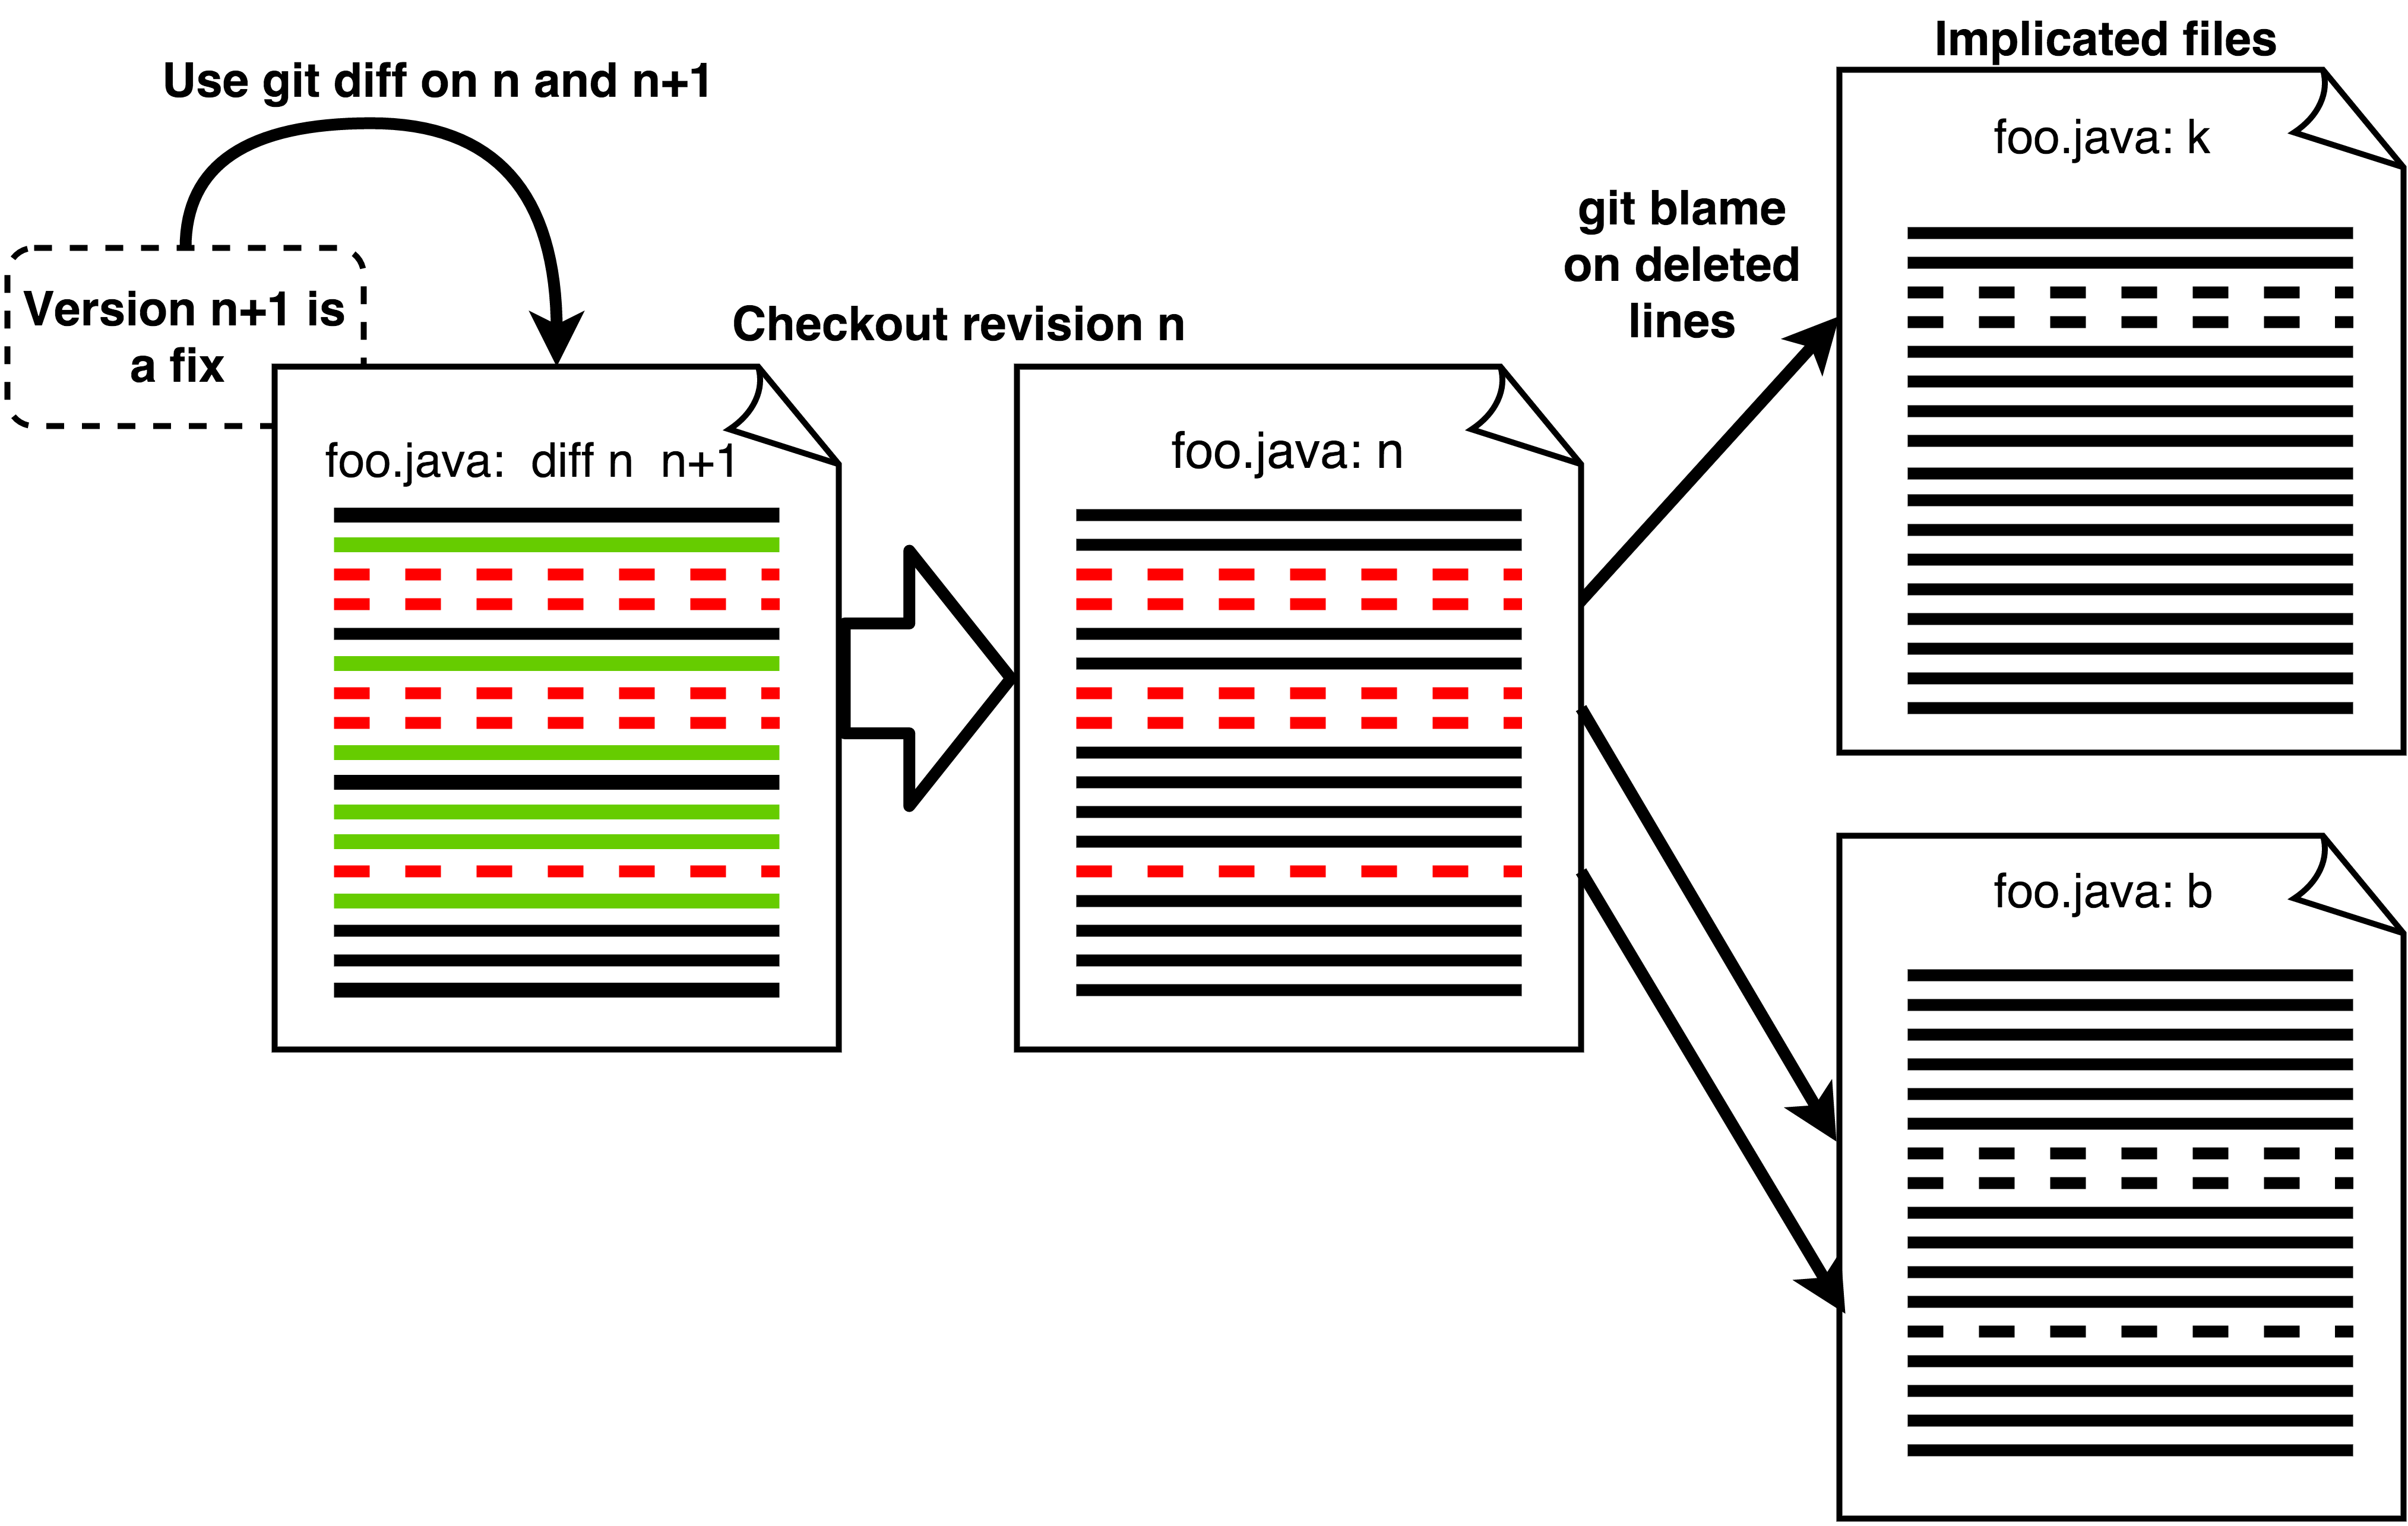
\includegraphics[width=\columnwidth]{images/implicated.png}
    \caption{Implicated code identification technique}
    \label{fig:implicated}
\end{figure}

In this work we don't consider the last step: this because we assume that if the lines are added after the issue reporting date, they are still based on a defective file, and so they contribute to the defect. We want to highlight the fact that a line of code is marked as implicated only in the version of the file in which it is introduced.

Since we need to spot defective file versions we define the new concept of \textbf{implicated file}: a file in a specific version is implicated if that version contains implicated code.

\subsection{Bug and commit linking technique}
\label{sec:bug-linking}
To apply the technique described to extract the implicated files we must be able to identify which commits are bug fixes. To do so we decided to use the JIRA issue tracking system~\footnote{\url{atlassian.com/software/jira}} and in particular the bug convention that Apache projects use on it~\footnote{\url{issues.apache.org/jira/secure/BrowseProjects.jspa\#all}}. Every Apache software project that uses JIRA has an issue key that is, by convention, mentioned in commits that address an issue, together with the issue id. In particular, the convention is to include these information with the following notation: KEY-ID (e.g. LUCENE-1234 if the commit addresses the issue 1234 of the Lucene project).

We consider a commit as a bug fix if its message mentions the key and id of an issue that is marked as a fixed bug on JIRA. To navigate through the JIRA issues we use the data extracted in JSON format in the work by

<MISSING: Cite the technical report for the JIRA JSON issues extraction.>


\subsection{Ownership metrics}
\label{sec:ownership-metrics}
As ownership metrics we decided to compute the ones defined by Bird et al.~\cite{bird:original} and already described in Section~\ref{sec:existing_solutions}. In particular we compute the first three ones (Ownership, Minor and Major) using three different variables to quantify code changes: commit count, number of lines added and number of lines deleted. We also use five different thresholds to distinguish minor and major contributors: 5\%, 10\%, 20\%, 30\% and 40\%. In this way we address also the second and the third of the problems described Section~\ref{sec:existing_solutions}.

To expand our study we also decided to compute the \textit{authorship}. Authorship can be seen as memory-less ownership: the metrics of this class are not based on the history of the development but only on the content of the file on which they are computed. The concept of authorship was already introduced by Rahman et al.~\cite{Rahman:blame}, but was applied only to implicated code chunks and not at a file level. In particular we  compute the two following metrics:
\begin{itemize}
    \item Line authorship: proportion of lines in the file authored by the developer with the highest proportion of lines authored;
    \item Total authors: total number of authors of the lines in the file.
\end{itemize}

We consider these two measures as part of our ownership metrics, following the memory-less vision described above.
To clarify the difference between the two classes of metrics lets suppose to compute them on the version V of the file F, using the number of lines added as variable to quantify the code changes:
\begin{itemize}
\item the proportion of ownership of the contributor C is computed as the number of lines added to F by C over all the considered history (all the versions of F that precede V), divided by the total number of lines added to F by all the contributors over all the considered history;
\item the proportion of authorship of the contributor C is computed as the number of lines that are actually in F in its version V and that are authored by C, divided by the size of F in the same version (in terms of lines);
\end{itemize}

\subsection{Classification}
\label{sec:classification-overview}
As already stated previously in this section, we use the concept of implicated code to mark code that can be considered defective, therefore in this research the defective files are the implicated ones. This means that the classification model that we want to build should distinguish which versions of the project files are implicated using the metrics that we described. 

To be able to evaluate our results in a way that is more sound in the defect prediction field, we first build a model that uses some classic code metrics that are known to be effective, then we add our metrics and we quantify the improvement in the model accuracy (a similar approach was also adopted by Bird et al.~\cite{bird:original}).

The classic metrics that we decided to use are (1) file size; (2) comment-to-code ratio; (3) number of previous defects (implications, in our case). We selected these three because are known to be indicative of software defects~\cite{Rahman:2013, d2012evaluating}.
\section{Methodology}

\subsection{Research questions}

We structure our research through the following research questions:

\begin{itemize}
    \item[\textbf{RQ1}] Are ownership metrics indicative for the presence of implicated code in source files for open-source software projects?
    
    \item[\textbf{RQ2}] Can ownership metrics be used to build a classification model to identify implicated source files?
    \begin{itemize}
        \item[\textbf{2a}] For which level of granularity (line-based or commit-based) do ownership metrics give more accurate results when used to build the classification model?
        \item[\textbf{2b}] How does the value of the threshold, used to distinguish minor and major contributors, impacts on the accuracy of the classification model?
    \end{itemize}
    % \item[\textbf{2a}] For which level of granularity (line-based or commit-based) do ownership metrics give more accurate results when used to build the classification model?
    
    % \item[\textbf{2b}] How does the value of the threshold, used to distinguish minor and major contributors, impacts on the accuracy of the classification model?
\end{itemize}

The first research question is a more general question, which is needed to determine if in general ownership metrics can be a good indication of the presence of implicated code in source files for open-source software. 
The second research question focuses on if it is possible to classify the implicated files based on ownership metrics. The sub-questions focus on the type of metrics included in the classifier: in particular on the parameters used to compute them (i.e. code changes granularity and minor-major threshold) and on the effects resulting from changing these parameters. %: which granularity (line or based) gives the best results, and if the minor-major threshold plays a significant role in classifying.

%In previous research, ownership has always been related to the amount of commits done by a specific contributor, but are there other ways to compute ownership that give a better result in terms of relationship with implicated files? The last research question focuses on the threshold to determine major or minor contributors. In previous research arbitrary values had been chosen for the threshold, but does have di

\subsection{Study subjects}
\label{sec:subjects}
A software project, in order to be used for this research, should (1) be and open-source software project; (2) use git as version control system, or have a git mirror of the repository (requirement for the technique described in Section~\ref{sec:implicated}; (3) use JIRA as issue tracking system and adhere to the Apache JIRA convention, so that we can apply the technique described in Section~\ref{sec:bug-linking}.

We selected five different software projects as study subjects, all written using the Java programming language. In Table~\ref{tab:projects} we show some information about each one of them. When choosing the projects we checked if they satisfied the previous mentioned requirements, but also tried to choose them with different sizes and application fields, in order to have a diverse group.

For each project we decided to  consider its whole development history until the 01/01/2015: this because we had issues extracted in JSON until the half of the year, and we only wanted to consider code for which the most of the issues were already discovered and fixed. We also decided to discard some of the first days of commits from the data extracted from the repositories, because these are the commits needed to setup the project repository or the git mirror. %As a result they commit sometimes years of data in one commit so the whole history there is lost. 
We did this last step by manually checking the messages of the first available commits.

\begin{table*}[ht]
\centering
\caption{Characteristics of the studied projects %over their history
(until 01/01/2015)}
\label{tab:projects}
\footnotesize
\begin{tabular}{|l|c|c|c|c|c|}
\hline
\textbf{Project} & \textbf{LOC} & \textbf{Contributors} & \textbf{Commits} & \textbf{Application} \\%& \textbf{Period}\\
\hline
Camel   & 103883  & 125 & 18371  & Rule-based routing and mediation engine \\
\hline
Lucene-solr & 220632 & 55 & 13841  & Information retrieval library and search platform\\
\hline
Mahout      & 177317 & 31 & 3163 &   Implementation of scalable machine-learning algorithms \\
\hline
Maven       & 129132 & 51 & 9909 &   Build manager \\
\hline
Zookeeper   & 108132 & 13  & 1283 &  Distributed system configuration service \\
\hline
\end{tabular}
\end{table*}


\subsection{Research steps}

What we want to do is to build a model that is able to identify the implicated files in the history of the selected software projects, and to evaluate its effectiveness. In this Section we describe in a detailed way all the steps followed in this research.

\subsubsection{Project history dataset}
\label{sec:history-dataset}

In the first step of our research we create, for every software project, a dataset that contains all its Java files history (over the considered time period, see Section~\ref{sec:subjects}) in terms of commits, lines, bug fixes and implications. To do that we go through all the commits in its \textit{git log}, and for every commit we:
\begin{enumerate}
\item extract the list of the Java files affected; 
\item for each affected file update the information about the contribution that the author of the commit performed to it in terms of lines added, lines deleted and number of commits;
\item extract information about the file itself: size (LOC), authorship information, comment lines, if it is a bug fix (using the technique described in Section~\ref{sec:bug-linking});
\item add to the data set, for each one of these files, as many lines as the number of authors that contributed to it until the considered commit (included): each one of these lines contains the information about the contribution of the corresponding author to the corresponding file, at the moment of the corresponding commit, plus the information related to the commit itself.
\end{enumerate}

We then add to this dataset, once extracted, another column that says when a file is implicated, using the approach described in Section~\ref{sec:implicated}.

A complete list of the columns contained in the dataset can be found in
\Cref{tab:modeled_information}. Some of them contain information that are not related to the single author, but to the file or the commit: in this case their value will be the same for more than one line.

An example of this procedure is shown in Figure~\ref{fig:history_example} and Table~\ref{tab:history_example}, it shows only information about commits and lines added but it can be used to better understand the described methodology.

\begin{figure}[ht]
    \centering
    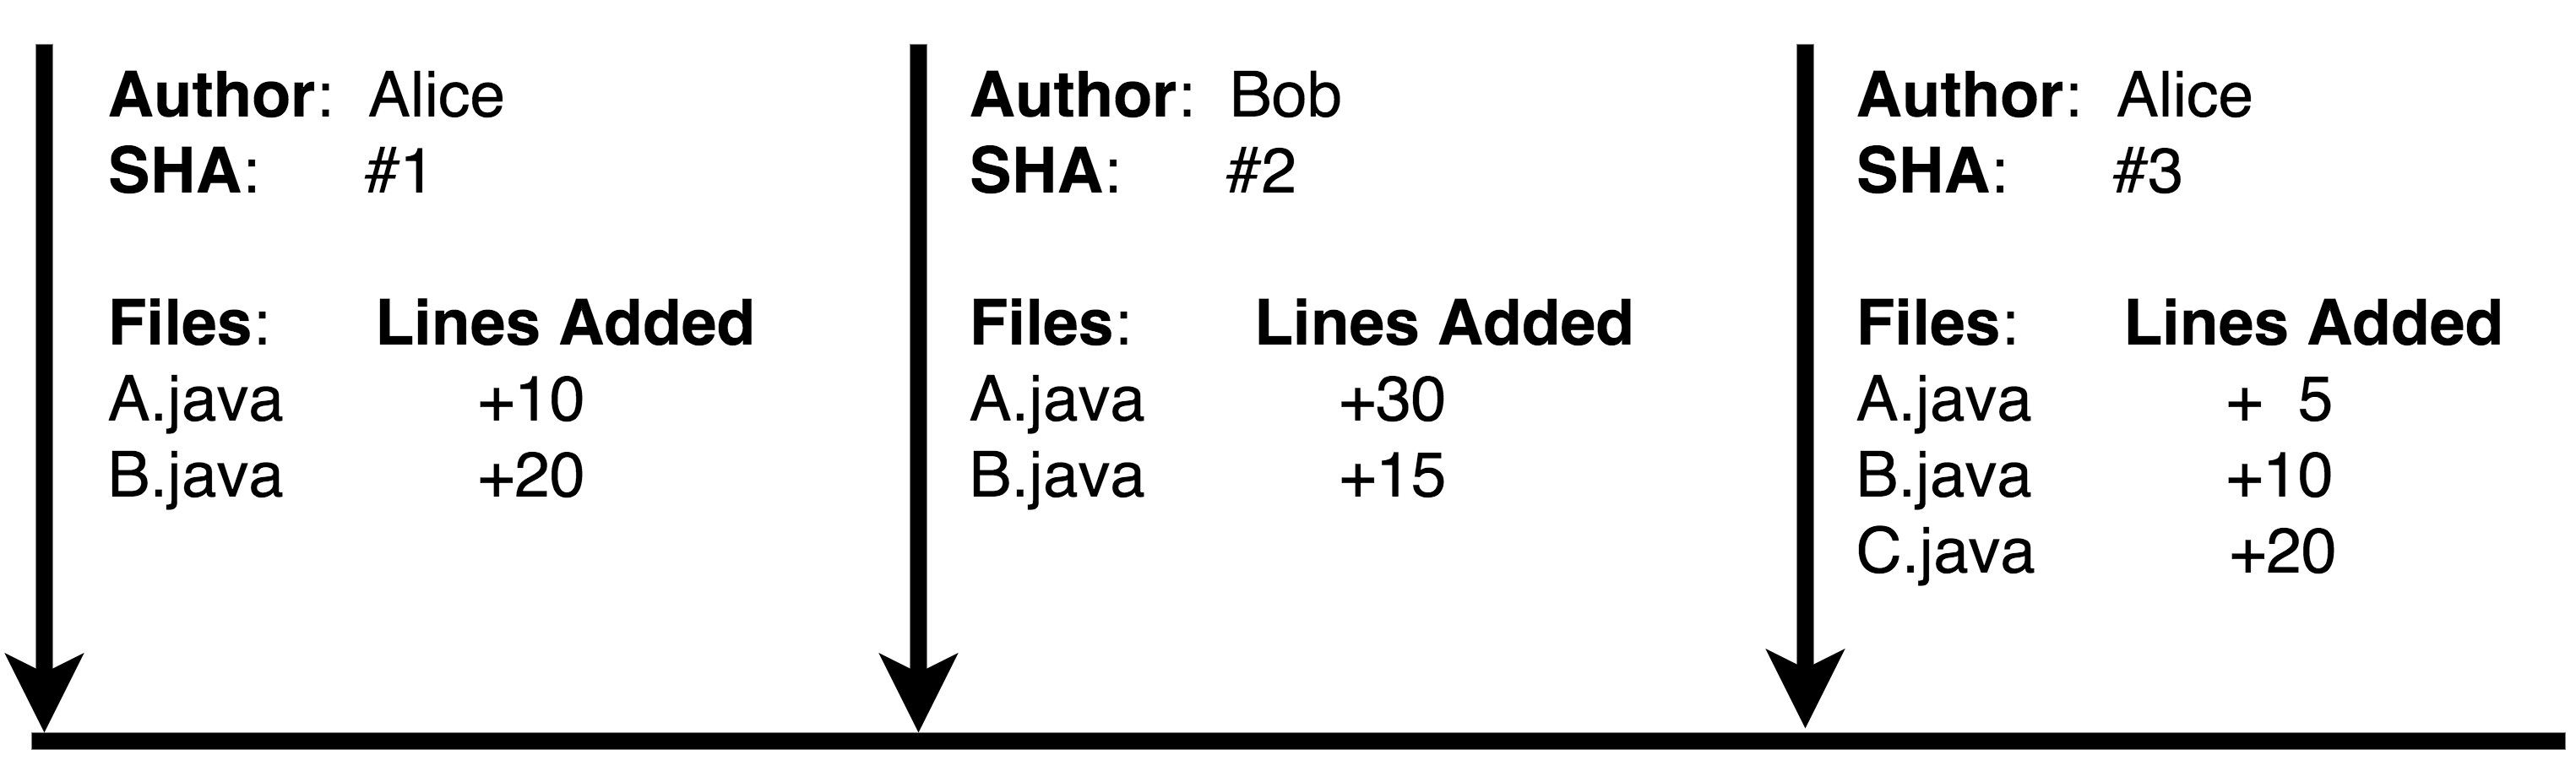
\includegraphics[width=0.48\textwidth]{images/history_example.png}
    \caption{Example of a small portion of development history (i.e. commits), with lines added information. The corresponding history dataset is shown in Table~\ref{tab:history_example}}
    \label{fig:history_example}
\end{figure}

\begin{table}[ht]
\centering
\footnotesize
\begin{tabular}{|c|c|c|c|c|c|c|c|}
\cline{3-8}
\multicolumn{1}{c}{} & 
\multicolumn{1}{c}{} & \multicolumn{6}{|c|}{\textbf{columns (see \Cref{tab:modeled_information})}} \\
\hline
\textbf{file} & \textbf{sha} & \textbf{4} & \textbf{5} & \textbf{6} & \textbf{7} & \textbf{11} & \textbf{12}
\\
\hline
A.java & \#1 & Alice  & 10                        & 10                                & 10               & 1                     & 1                  \\
B.java & \#1 & Alice  & 20                        & 20                                & 20               & 1                     & 1                  \\
A.java & \#2 & Alice  & 10                        & 0                                 & 40               & 1                     & 2                  \\
A.java & \#2 & Bob    & 30                        & 30                                & 40               & 1                     & 2                  \\
B.java & \#2 & Alice  & 20                        & 0                                 & 35               & 1                     & 2                  \\
B.java & \#2 & Bob    & 15                        & 15                                & 35               & 1                     & 2                  \\
A.java & \#3 & Alice  & 15                        & 5                                 & 45               & 2                     & 3                  \\
A.java & \#3 & Bob    & 30                        & 0                                 & 45               & 1                     & 3                  \\
B.java & \#3 & Alice  & 30                        & 10                                & 45               & 2                     & 3                  \\
B.java & \#3 & Bob    & 15                        & 0                                 & 45               & 1                     & 3                  \\
C.java & \#3 & Alice  & 20                        & 20                                & 20               & 1                     & 1 \\\hline
\end{tabular}
\caption{Example of a small portion of history dataset with a reduced set of columns. The corresponding development history is shown in Figure~\ref{fig:history_example}}.
\label{tab:history_example}
\end{table}

\begin{table}[ht]
\centering
\footnotesize
\begin{tabular}{|c|c|c|c|c|c|c|c|c|}
\cline{3-9}
\multicolumn{1}{c}{} & 
\multicolumn{1}{c}{} & \multicolumn{7}{|c|}{\textbf{columns (see Table~\ref{tab:metrics})}} \\
\hline
\textbf{sha} & \textbf{file} & \textbf{3} & \textbf{4} & \textbf{6} & \textbf{11} & \textbf{12} & \textbf{13} & \textbf{14}
\\
\hline
\#1 & A.java & 1 / 1             & 10 / 10                & 1                   & 1                   & 0                   & 1                                 & 0                                 \\
\#1 & B.java & 1 / 1             & 20 / 20                & 1                   & 1                   & 0                   & 1                                 & 0                                 \\
\#2 & A.java & 1 / 2             & 30 / 40                & 2                   & 2                   & 0                   & 1                                 & 1                                 \\
\#2 & B.java & 1 / 2             & 20 / 35                & 2                   & 2                   & 0                   & 2                                 & 0                                 \\
\#3 & A.java & 2 / 3             & 30 / 45                & 2                   & 2                   & 0                   & 2                                 & 0                                 \\
\#3 & B.java & 2 / 3             & 30 / 45                & 2                   & 2                   & 0                   & 2                                 & 0                                 \\
\#3 & C.java & 1 / 1             & 20 / 20                & 1                   & 1                   & 0                   & 1                                 & 0                 
\\ \hline
\end{tabular}
\caption{Example of a small portion of metrics dataset with a reduced set of columns, extracted from the history dataset example shown in Table~\ref{tab:history_example} using a 30\% threshold to distinguish minor and major contributors.}
\label{tab:metrics_example}
\end{table}

\begin{table*}[ht]
\centering
\caption{Information modeled and stored in our dataset, per committed file}
\label{tab:modeled_information}
\begin{tabular}{|l|l|p{0.65\textwidth}|}
\hline
\# & \textbf{Column} & \textbf{Description}  \\\hline
\hline
1 & project & 
    project name \\ \hline
2 & file & 
    file name (full path)\\ \hline
3 & sha & 
    commit SHA (also, file revision) \\ \hline
4 & author & 
    contributor's name \textbf{(NOTE: it is not the author of the commit, but one of the file contributors)} \\ \hline
5 & author\_file\_tot\_added & 
    total lines added by the author to the file\\ \hline
6 & author\_file\_added\_this\_commit & 
    lines added by the author to the file with the commit (different from 0 only for the author of the commit)\\ \hline
7 & file\_tot\_added & 
    total lines added to the file\\ \hline
8 & author\_file\_tot\_deleted & 
    total lines deleted by the author from the file\\ \hline
9 & author\_file\_deleted\_this\_commit & 
    lines deleted by the author from the file with the commit (different from 0 only for the author of the commit)\\ \hline
10 & file\_tot\_deleted & 
    total lines deleted from the file\\ \hline
11 & author\_file\_commits & 
    total commits to the file by the author\\ \hline
12 & file\_tot\_commits & 
    total commits to the file\\ \hline
13 & current\_lines\_authored & 
    number of lines actually present in the file and authored by the author (obtained from the \textit{git blame} output)\\\hline
14 & current\_file\_size & 
    file size measured in LOC (lines of code)\\\hline
15 & current\_comment\_lines & 
    comments size in terms of lines\\\hline
16 & max\_current\_author & 
    number of lines actually present in the file and authored by the author that authored the highest number of lines actually in the file (obtained from the \textit{git blame} output)\\\hline
17 & total\_current\_authors & 
    number of authors of the lines actually present in the file (obtained from the \textit{git blame} output)\\\hline
18 & commit\_date & date of the commit\\ \hline
19 & bug\_fix & 1 if the commit fixes one or more bugs, zero otherwise\\ \hline
20 & fixed\_bugs & JIRA KEY-ID of the bugs fixed, empty if the commit is not a bug fix\\ \hline
21 & affected\_versions & list of the project releases affected by the bugs fixed by the commit, empty if the commit is not a bug fix\\ \hline
22 & implicated & 1 if the file version is implicated \\ \hline
\end{tabular}
\end{table*}


\subsubsection{Metrics computation}
\label{sec:metrics}
In this second step, for every project and using the respective history
dataset, we compute the dataset that contain the metrics that we need for the
classification. We need to compute the metrics for every version of every file,
so the computation is done grouping by commit SHA and file (columns 2 and 3 of
the history dataset, see \Cref{tab:modeled_information}). 

As metrics we compute the ownership ones described in
Section~\ref{sec:ownership-metrics} together with the classic code metrics
listed in Section~\ref{sec:classification-overview}. This will produce another
data set, with fewer lines, that contains the metrics and the column
``implicated'', defined as in \Cref{tab:modeled_information}. A complete set of the columns of the metrics dataset can be seen in Table~\ref{tab:metrics}, where the terms ownership, minor, major and total must be interpreted as defined in Section~\ref{sec:ownership-metrics}. 

A different version of this dataset is computed for every threshold listed in Section~\ref{sec:ownership-metrics} (the threshold used to distinguish minor and major contributors).
Table~\ref{tab:metrics_example} shows an example of the metrics dataset resulting from the history dataset example shown in Table~\ref{tab:history_example}, using a threshold of 30\%; it contains a reduced set of columns: only the ones based on the lines added and on the commit count.

\begin{table*}[t]
\centering
\caption{Columns of the metrics dataset;  See
Section~\ref{sec:ownership-metrics} and \Cref{tab:modeled_information} for the terms used in the definitions.}
\label{tab:metrics}
\footnotesize
\begin{tabular}{|l|l|p{0.65\textwidth}|}
\hline
\# & \textbf{Column} & \textbf{Description}  \\
\hline
1 & sha & 
    commit SHA (can be interpreted as file version or revision) \\ \hline
2 & file & 
    file name (full path)\\ \hline
3 & commit\_ownership & 
    max( author\_file\_commits / file\_tot\_commits)\\ \hline
4 & line\_ownership\_added & 
    max( author\_file\_tot\_added / file\_tot\_added)\\ \hline
5 & line\_ownership\_deleted & 
    max( author\_file\_tot\_deleted / file\_tot\_deleted)\\ \hline
6 & total\_contributors & 
    total number of contributors (count the of the lines grouped together) \\ \hline %since for a specific file and sha there are as many lines as the number of contributors in the history dataset)
7 & line\_authorship & 
    max\_current\_author / file\_size \\ \hline
8 & total\_authors & 
    total\_current\_authors\\ \hline
9 & file\_size & 
    file\_size\\ \hline
10 & comment\_to\_code\_ratio & 
    current\_comment\_lines / (current\_file\_size - current\_comment\_lines)\\ \hline
11 & major\_contributors & 
    count where author\_file\_commits / file\_tot\_commits >= threshold\\ \hline
12 & minor\_contributors & 
    count where author\_file\_commits / file\_tot\_commits < threshold\\ \hline
13 & lines\_added\_major\_contributors & 
    count where author\_file\_tot\_added / file\_tot\_added >= threshold\\ \hline
14 & lines\_added\_minor\_contributors & 
    count where author\_file\_tot\_added / file\_tot\_added < threshold\\ \hline
15 & lines\_deleted\_major\_contributors & 
    count where author\_file\_tot\_deleted / file\_tot\_deleted >= threshold\\ \hline
16 & lines\_deleted\_minor\_contributors & 
    count where author\_file\_tot\_deleted / file\_tot\_deleted < threshold\\ \hline
17 & previous\_implications &
    count how many times this file was implicated before that version\\\hline
18 & implicated & 1 if the file version is implicated \\\hline
\end{tabular}
\end{table*}

\subsubsection{Classification}
Using the metrics dataset we build, for every project, a classification model using the Random Forests approach~\cite{breiman2001random}, and we then evaluate how effective it is when used to distinguish which file versions are implicated. We also use Logistic Regression to determine which features are significant. The choice of these techniques is based on the fact that they were already used respectively in~\cite{Greiler:replication} and~\cite{bird:original}. An accurate description of this process is provided in Section~\ref{sec:evaluation}.


% Correlation and classification of buggy files/commits.
%\subsubsection{Statistical approach}
%The features will be used to see if there is a correlation between them and the fact that a file is implicated. For the classification we will use the \textit{Random Forest} classification algorithm.



% Compute metrics for all commits and all files changed by that commit

% Find all implicated code by finding all fixing commits and using git diff and blame to find the commits when those lines where last modified.


% New data set (for the Lucene projects) that contains:
% - All the history of the commits
% For every commit, all the files changed
% For every file changed, author ownership (at the time of the commit) and bug information (implicated, fix, etc.)
% Ownership metrics computation (different granularities) and Exploratoty Data Analysis → determine minor / major threshold
% Correlations and classification of buggy files/commits
% Replicate on more OSS projects



% The dataset of every project contains several field, which contain data specific to the commit, file, and author. The dataset contain the following fields:



% From this dataset different kinds of ownership metrics will be extracted, which will be used to find a correlation with code quality.[h

\section{Evaluation}
\label{sec:evaluation}
% for LOC run: git ls-files | grep  \.java | xargs wc -l | awk '{ SUM += $1} END { print SUM }'
% for Commits run: bug_column_blame_approach, and then take len(commits) of each project
% for # of contributers (assuming unique), "git checkout --force master" and  "git shortlog -s -n | wc -l"
% for # of commits : git rev-list --count trunk

\subsection{Experiment 1: Ownership and granularity}

\subsubsection{Experiment design}

In this experiment we address research questions 1 and 2 building a model that can classify implicated files using the classic code metrics, and evaluating if the ownership metrics can improve its effectiveness. We also address question 2a comparing the improvement given by different ownership granularities (commit-based and line-based).

\begin{table}[ht]
    \footnotesize
    \centering
    \caption{Class sample size per project}
    \label{tab:sample_size}
    \begin{tabular}{|c|c|c|}
        \hline
        \textbf{Project} & \textbf{Implicated files} & \textbf{Sample size} \\
        \hline
        Camel & 7076 & 4000 \\
        Lucene-Solr & 14416 & 4000 \\
        Mahout & 2114 & 2000 \\
        Maven  & 2383 & 2000 \\
        Zookeeper & 819 & 800 \\
        \hline
    \end{tabular}
\end{table}

This experiment is performed for every considered project using its metrics dataset with the 5\% threshold. We define different subsets of features (see Table~\ref{tab:metric_groups}), and for each one of them we cross-validate (10-folds) the Random Forest~\cite{breiman2001random} model on a sample of the dataset. The sample contains the same number of lines for both the classes (implicated and not implicated, see Table~\ref{tab:sample_size}).


\begin{table}[ht]
    \centering
    \footnotesize
    \caption{Considered set of metrics}
    \label{tab:metric_groups}
    \begin{tabular}{|c|p{0.3\textwidth}|}
        \hline
        \textbf{Group} & \textbf{Metrics} \\
        \hline
        Classic & file\_size, comment\_to\_code\_ratio, previous\_implications \\
        \hline
        Commit based & Classic + commit\_ownership, minor\_contributors, major\_contributors \\
        \hline
        Deleted  & Classic + line\_ownership\_deleted, lines\_deleted\_minor\_contributors, lines\_deleted\_major\_contributors \\
        \hline
        Added  & Classic + line\_ownership\_added, lines\_added\_minor\_contributors, lines\_added\_major\_contributors,\\
        \hline
        Line authorship  & Classic + line\_authorship, total\_authors\\
        \hline
        Line based  & Classic + Added + Deleted \\
        \hline
        All metrics  & All the above mentioned metrics minus the highly correlated ones (cutoff=0.75)\\
        \hline
    \end{tabular}
\end{table}

We evaluate the constructed classifiers with the out-of-bag error rate (OOB) averaged over the 10-folds, and use it to determine if the improvement over the classic metrics is statistically significant. This is done by comparing with the t-test the outcome of every set of metrics with the outcome obtained considering only the classic ones. For the test we assume a significance level of \textit{0.05}.


\subsubsection{Results}

In Table \ref{tab:granularity_lucene} the results for the project Lucene-Solr can be found. It can be noted here that the different granularities between metrics have a significant influence on the performance of the classifier. Line-based metrics (deleted, added, authorship) give a larger performance increase than the commit-based ones. This effect is highlited also in Figure~ \ref{fig:importance_var_lucene}: it shows the importance of the single metrics for Lucene-Solr. Eventually, Figure~\ref{fig:roc_lucene} shows the corresponding ROC curve. Similar results come from the other projects.

Table \ref{tab:sum_experiment_1_results} shows a summary of the results of the experiment. Using all the metrics the average OOB is 22.99\% which gives an average increase of 21.71\%  in performance over the classic metrics. For what concerns the granularity, line-based metrics perform on average 15\% better than commit-based metrics.
All the p-values resulting from the significance test performed on the improvements are far below the 0.05 significance level, meaning that all the improvements over the classic metrics are statistically significant.


% \begin{table}[ht]
% \centering
% \footnotesize
% \caption{Lucene-Solr experiment 1 results}
% \label{tab:granularity_lucene}
% \begin{tabular}{|c|c|c|}
% \hline
% \textbf{Features} & \textbf{\begin{tabular}[c]{@{}c@{}}OOB with\\ 5\% threshold\end{tabular}} & \textbf{\begin{tabular}[c]{@{}c@{}}Improvement\\ over Classic\end{tabular}} \\ \hline
% Classic & 32.39\% & 0.00\%  \\
% \hline
% \begin{tabular}[c]{@{}c@{}}Classic +\\ Commit based\end{tabular} &  30.65\% & 5.66\%  \\
% \hline
% \begin{tabular}[c]{@{}c@{}}Classic +\\ Deleted\end{tabular} & 29.42\% & 10.10\% \\
% \hline
% \begin{tabular}[c]{@{}c@{}}Classic +\\ Added\end{tabular} & 29.88\% & 8.41\%  \\
% \hline
% \begin{tabular}[c]{@{}c@{}}Classic +\\ Line authorship\end{tabular} & 29.26\% & 10.68\% \\
% \hline
% \begin{tabular}[c]{@{}c@{}}Classic +\\ Line based\end{tabular} & 26.15\% & 23.84\% \\
% \hline
% All metrics & 26.11\% & 24.04\% \\
% \hline
% \end{tabular}
% \end{table}

\begin{table*}[ht]
\centering
\footnotesize
\caption{Lucene-Solr experiment 1 results}
\label{tab:granularity_lucene}
\begin{tabular}{|c|c|c|c|c|}
\hline
\textbf{Features} & \textbf{\begin{tabular}[c]{@{}c@{}}Error Rate\\ with 5\% threshold\end{tabular}} & \textbf{\begin{tabular}[c]{@{}c@{}}Improvement\\ over Classic\end{tabular}} & \textbf{Precision} & \textbf{Recall} \\
\hline
Classic & 32.59\% & 0.00\% & 67.85\% & 67.26\% \\
\hline
\begin{tabular}[c]{@{}c@{}}Classic +\\ Commit based\end{tabular} & 30.38\% & 6.78\% & 67.21\% & 70.62\% \\
\hline
\begin{tabular}[c]{@{}c@{}}Classic +\\ Deleted\end{tabular} & 29.69\% & 8.88\% & 70.09\% & 70.40\% \\
\hline
\begin{tabular}[c]{@{}c@{}}Classic +\\ Added\end{tabular} & 29.49\% & 9.51\% & 69.40\% & 70.98\% \\
\hline
\begin{tabular}[c]{@{}c@{}}Classic +\\ Line authorship\end{tabular} & 29.46\% & 9.59\% & 74.29\% & 69.11\% \\
\hline
\begin{tabular}[c]{@{}c@{}}Classic +\\ Line based\end{tabular} & 26.12\% & 19.86\% & 80.41\% & 71.13\% \\
\hline
All metrics & 26.34\% & 19.16\% & 80.50\% & 70.81\% \\
\hline
\end{tabular}
\end{table*}


% \begin{table}[ht]
% \centering
% \caption{Summary of the results of experiment 1}
% \label{tab:sum_experiment_1_results}
% \begin{tabular}{|c|c|c|c|}
% \hline
% \textbf{Project} & \textbf{Classic} & \textbf{All metrics} & \textbf{Improvement} \\
% \hline
% Lucene-Solr      & 32.39\%          & 26.11\%              & 24.04\%              \\
% Mahout           & 29.50\%          & 14.65\%              & 101.33\%             \\
% Camel            & 32.35\%          & 26.40\%              & 22.51\%              \\
% Maven            & 26.39\%          & 19.33\%              & 36.49\%              \\
% Zookeeper        & 24.31\%          & 20.00\%              & 21.53\%              \\
% \hline
% \textbf{Average} & \textbf{28.99\% }         & \textbf{21.30\%}              & \textbf{41.18\% }   \\
% \hline
% \end{tabular}
% \end{table}

\begin{table*}[ht]
\centering
\caption{Summary of the results of experiment 1}
\label{tab:sum_experiment_1_results}
\begin{tabular}{|c|c|c|c|c|c|c|}
\hline
\textbf{Project} & \textbf{Classic} & \textbf{Commit based} & \textbf{Line based} & \textbf{All metrics} & \textbf{\begin{tabular}[c]{@{}c@{}}Improvement\\ (all metrics with FS)\end{tabular}} & \textbf{\begin{tabular}[c]{@{}c@{}}Improvement\\ (Line based)\end{tabular}} \\
\hline
lucene-solr & 32.59\% & 30.38\% & 26.12\% & 26.34\% & 19.16\% & 19.86\% \\
mahout & 31.68\% & 29.44\% & 25.42\% & 29.33\% & 7.43\% & 19.77\% \\
Camel & 29.36\% & 25.16\% & 19.38\% & 19.25\% & 34.43\% & 34.00\% \\
Maven & 25.51\% & 23.19\% & 19.27\% & 19.09\% & 25.15\% & 24.45\% \\
Zookeeper & 26.94\% & 22.35\% & 20.67\% & 20.92\% & 22.37\% & 23.27\% \\
\hline
Average & 29.22\% & 26.10\% & 22.17\% & 22.99\% & 21.71\% & 24.27\%\\
\hline
\end{tabular}
\end{table*}

\begin{figure}
    \centering
    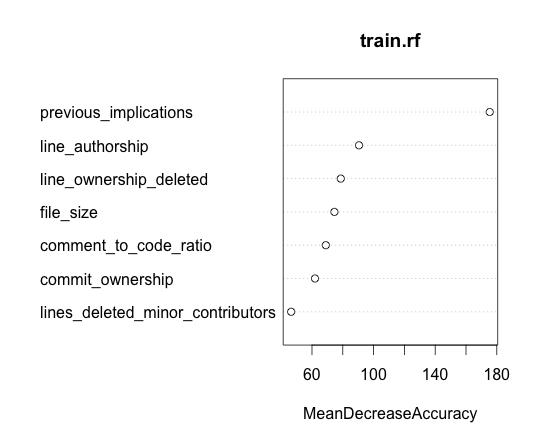
\includegraphics[width=0.45\textwidth]{images/lucene_importance_2.png}
    \caption{Importance of variables for Lucene-Solr}
    \label{fig:importance_var_lucene}
\end{figure}


%  \ref{fig:importance_var_mahout} \ref{fig:importance_var_camel} \ref{fig:importance_var_maven} \ref{fig:importance_var_zookeeper}
% \begin{figure}
%     \centering
%     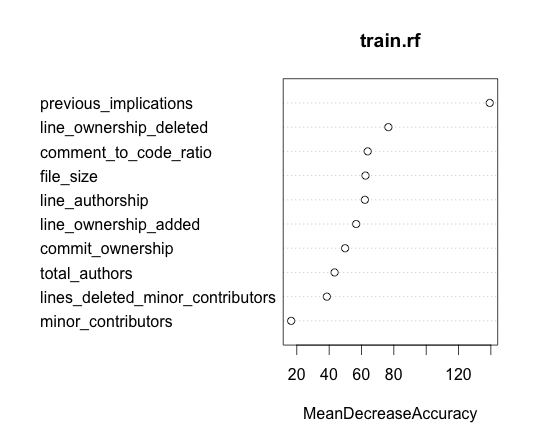
\includegraphics[width=0.45\textwidth]{images/mahout_importance_2.png}
%     \caption{Importance of variables for Mahout}
%     \label{fig:importance_var_mahout}
% \end{figure}

% \begin{figure}
%     \centering
%     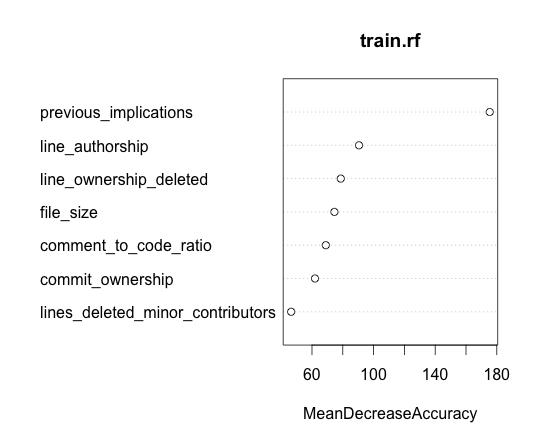
\includegraphics[width=0.45\textwidth]{images/camel_importance_2.png}
%     \caption{Importance of variables for Camel}
%     \label{fig:importance_var_camel}
% \end{figure}

% \begin{figure}
%     \centering
%     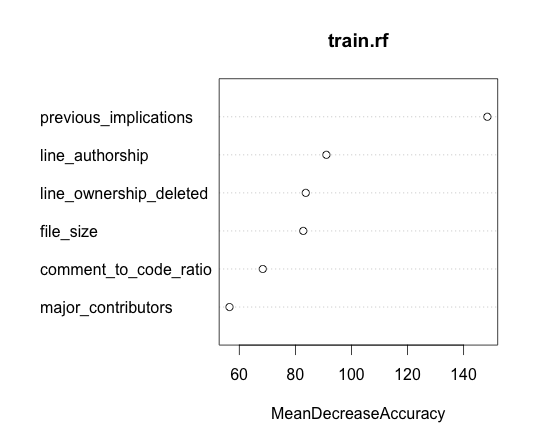
\includegraphics[width=0.45\textwidth]{images/maven_importance_2.png}
%     \caption{Importance of variables for Maven}
%     \label{fig:importance_var_maven}
% \end{figure}

% \begin{figure}
%     \centering
%     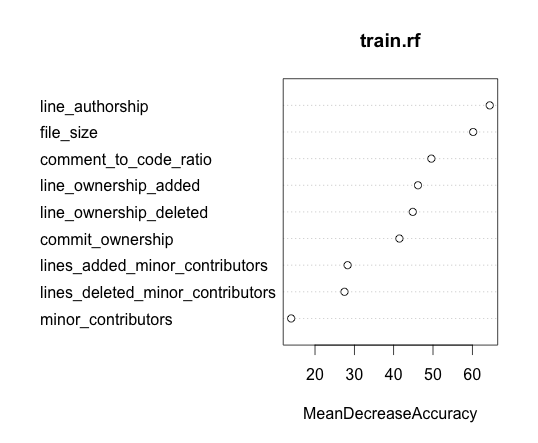
\includegraphics[width=0.45\textwidth]{images/zookeeper_importance_2.png}
%     \caption{Importance of variables for Zookeeper}
%     \label{fig:importance_var_zookeeper}
% \end{figure}

\begin{figure}[ht]
    \centering
    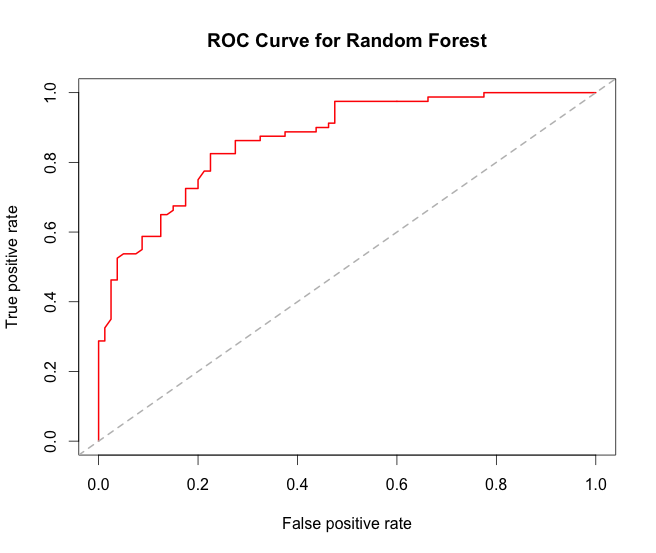
\includegraphics[width=0.45\textwidth]{images/ROC_lucene_05_all.png}
    \caption{ROC curve resulting from experiment 1 on Lucene-Solr, considering all the metrics.}
    \label{fig:roc_lucene}
\end{figure}


\subsection{Experiment 2: Logistic regression}

\subsubsection{Experiment design}

In the previous experiment we used Random Forest to determine the performance of different granularities. In this experiment we will take it a step further by taking a look at the individual metrics to see how statistically significant they are. The goal is to determine which metrics are significant, checking also if the significance changes depending on the threshold, and to determine if there is a common group of metrics that is significant for all the selected study subjects.

We determine the statistically significant metrics by running Logistic Regression on the dataset without feature selection, since this technique automatically detects which ones are not linearly dependent with each other. Logistic regression is a good choice in this case: this because it automatically computes the significance of every variable in terms of p-value.


\begin{table}[ht]
\centering
\caption{Logistic Regression outcomes explanation.}
\label{tab:significant_sym}
\begin{tabular}{cc}
\hline
Pr(>|z|) & Symbol \\
\hline
0       & $\ast\ast\ast$      \\
0.001   & $\ast\ast$          \\
0.01    & $\ast$              \\
0.05    & .                   \\
0.1     &  \\
NA      & NA\\
\hline
\end{tabular}
\end{table}

\subsubsection{Results}

Table~\ref{tab:significant_sym} shows how to interpret the results of the Logistic Regression:  NA means that the metric is considered linearly dependent with another one and because of that it is not taken into consideration. Table~\ref{tab:logistic_regression5} summarizes the results of the significance of the different metrics for the 5\% threshold.

The classic metrics are, as expected, highly significant. It can be noted that the total contributors and line authorship are also highly significant for all the projects, while the rest of the ownership metrics significance values vary a lot, meaning they are probably more project dependent. Despite that, for every project it is possible to see that at least five of these ownership metrics are statistically significant (considering a 0.05 significance level).

Table \ref{tab:experiment2_threshold} shows the influence that changing the threshold has on the significance. It can be seen there is no clear improvement in significance for the metrics, meaning that when the threshold changes the change in the significance of the metrics is not relevant: while some of them become more significant, others result to be less important. For example, when considering a 10\% threshold, \textit{lines\_added\_major\_contributors} becomes more significant for Lucene-Solr but also less significant for Mahout, in comparison to the 5\% threshold scenario. For other threshold values the results are similar.


\begin{table*}[ht]
\centering
\caption{Results of logistic regression with the metrics with a 5\% threshold, see Table~\ref{tab:significant_sym} for the interpretation.}
\label{tab:logistic_regression5}
\begin{tabular}{|c|c|c|c|c|c|}
\hline
\textbf{Metrics}                 & \textbf{Lucene-Solr} & \textbf{Camel} & \textbf{Mahout} & \textbf{Maven}  & \textbf{Zookeeper} \\ \hline
file size                        & \textbf{$\ast\ast\ast$}         & \textbf{$\ast\ast\ast$}   & \textbf{$\ast\ast\ast$}    & \textbf{$\ast\ast\ast$}    &                    \\
previous implications            & \textbf{$\ast\ast\ast$}         & \textbf{$\ast\ast\ast$}   & \textbf{$\ast\ast\ast$}    & \textbf{$\ast\ast\ast$}    & \textbf{$\ast\ast\ast$}       \\
comment to code ratio            & \textbf{.}           & \textbf{$\ast\ast\ast$}   & \textbf{$\ast\ast\ast$}    & \textbf{$\ast\ast\ast$}    & \textbf{$\ast\ast\ast$}       \\
\hline
commit ownership                 &                      & \textbf{$\ast\ast\ast$}   & \textbf{$\ast$}      & \textbf{$\ast\ast\ast$}    & \textbf{.}         \\
minor contributors               & NA                   & NA             & \textbf{$\ast\ast$}     & NA              & NA                 \\
major contributors               & \textbf{$\ast\ast\ast$}         & \textbf{$\ast\ast\ast$}   & NA              & \textbf{$\ast\ast\ast$}    & \textbf{$\ast\ast\ast$}       \\
total contributors & \textbf{$\ast\ast\ast$} & \textbf{$\ast\ast\ast$} & \textbf{$\ast\ast\ast$} & \textbf{$\ast\ast\ast$} & \textbf{$\ast\ast\ast$} \\\hline
total authors                    & \textbf{$\ast\ast\ast$}         & \textbf{}      & \textbf{}       & \textbf{}       & \textbf{$\ast\ast\ast$}       \\
line authorship                  & \textbf{$\ast\ast\ast$}         & \textbf{$\ast\ast\ast$}   & \textbf{$\ast\ast\ast$}    & \textbf{$\ast\ast\ast$}    & \textbf{$\ast\ast\ast$}       \\ \hline
line ownership added             & \textbf{}            & \textbf{$\ast\ast\ast$}   & \textbf{$\ast\ast\ast$}    & \textbf{$\ast\ast\ast$}    & \textbf{.}         \\
lines added minor contributors   & \textbf{}            & NA             & \textbf{}       & NA              & NA                 \\
lines added major contributors   & \textbf{}            & \textbf{$\ast\ast$}    & \textbf{.}      & \textbf{}       & \textbf{$\ast\ast$}        \\ \hline
line ownership deleted           & \textbf{.}           & \textbf{$\ast\ast\ast$}   & \textbf{$\ast\ast\ast$}    & \textbf{}       & \textbf{.}         \\
lines deleted minor contributors & NA                   & NA             &                 & NA              & NA                 \\
lines deleted major contributors & \textbf{$\ast$}           & \textbf{}      & \textbf{$\ast$}      & \textbf{$\ast\ast$}     & \textbf{}          \\ \hline
\textbf{Accuracy}                & \textbf{0.6325}      & \textbf{0.65}  & \textbf{0.6925} & \textbf{0.6425} & \textbf{0.59375}   \\ \hline
\end{tabular}
\end{table*}



\begin{table*}[ht]
\centering
\caption{Major contributors metrics with different granularities and the influence of the threshold for different projects}
\label{tab:experiment2_threshold}
\begin{tabular}{|c|c|c|c|c|c|c|}
\hline
\textbf{Threshold} & \textbf{Metrics} & \textbf{Lucene-solr} & \textbf{Camel} & \textbf{Mahout} & \textbf{Maven} & \textbf{Zookeeper} \\
\hline
\multirow{3}{*}{5\%} & major contributors & \textbf{$\ast\ast\ast$} & \textbf{$\ast\ast\ast$} & NA & \textbf{$\ast\ast\ast$} & \textbf{$\ast\ast\ast$} \\
 & lines added major contributors & \textbf{} & \textbf{$\ast\ast$} & \textbf{.} & \textbf{} & \textbf{$\ast\ast$} \\
 & lines deleted major contributors & \textbf{$\ast$} & \textbf{} & \textbf{$\ast$} & \textbf{$\ast\ast$} & \textbf{} \\
\hline
\multirow{3}{*}{10\%} & major contributors & \textbf{$\ast\ast\ast$} & \textbf{} & \textbf{} & \textbf{} & \textbf{$\ast\ast\ast$} \\
 & lines added major contributors & \textbf{$\ast\ast$} & \textbf{$\ast\ast\ast$} & \textbf{} & \textbf{$\ast\ast$} & \textbf{$\ast\ast\ast$} \\
 & lines deleted major contributors & \textbf{} & \textbf{} & \textbf{} & \textbf{$\ast\ast\ast$} & \textbf{} \\
\hline
\multirow{3}{*}{20\%} & major contributors & \textbf{$\ast\ast\ast$} & \textbf{$\ast\ast$} & \textbf{$\ast\ast$} & \textbf{$\ast\ast\ast$} & \textbf{.} \\
 & lines added major contributors & \textbf{$\ast\ast\ast$} & \textbf{} & \textbf{.} & \textbf{} & \textbf{} \\
 & lines deleted major contributors & \textbf{} & \textbf{} & \textbf{$\ast\ast\ast$} & \textbf{$\ast\ast\ast$} & \textbf{} \\
\hline
\multirow{3}{*}{30\%} & major contributors & \textbf{$\ast\ast\ast$} & \textbf{} & \textbf{$\ast$} & \textbf{} & \textbf{} \\
 & lines added major contributors & \textbf{$\ast\ast\ast$} & \textbf{$\ast\ast\ast$} & \textbf{$\ast\ast$} & \textbf{} & \textbf{} \\
 & lines deleted major contributors & \textbf{} & \textbf{} & \textbf{$\ast\ast\ast$} & \textbf{$\ast\ast\ast$} & \textbf{} \\
\hline
\multirow{3}{*}{40\%} & major contributors & \textbf{$\ast\ast\ast$} & \textbf{} & \textbf{$\ast\ast$} & \textbf{$\ast$} & \textbf{} \\
 & lines added major contributors & \textbf{$\ast\ast\ast$} & \textbf{$\ast\ast\ast$} & \textbf{$\ast\ast$} & \textbf{} & \textbf{.} \\
 & lines deleted major contributors & \textbf{} & \textbf{} & \textbf{$\ast$} & \textbf{$\ast\ast\ast$} & \textbf{}\\
 \hline
\end{tabular}
\end{table*}




\subsection{Experiment 3: Minor-major thresholds}

\subsubsection{Experiment design}

Research question 2b has to do with the threshold used to distinguish minor and major contributors and with how much does it influence the performance of the classifier. The goal of the experiment is to determine the effect of the different thresholds that we selected to use: \texttt{0.05}, \texttt{0.10}, \texttt{0.20}, \texttt{0.30}, and \texttt{0.40}.

As said in Section~\ref{sec:metrics}, for every project we computed a metrics dataset for each one of the thresholds. In this experiment we use again the Random Forest technique to build a classifier for every threshold and every project, considering only the metrics that depend on the threshold, so all the ones that measure minor and major contributors (see Table~\ref{tab:metrics}). This results in 25 classifiers.

The performance of every classifier is measured using 10-folds cross-validation and the OOB error: since we used only features that depend from the threshold, the difference between these resulting models is only related to its variation.

To determine if the 5 groups of OOB errors, corresponding to different thresholds, differ in a statistically significant way we apply an \textit{ANOVA} test, which will tell if the outcomes are statistically significant. Based on the output p-values we can determine if some thresholds are statistically better than other ones for some of the projects.


\subsubsection{Results}

In Table \ref{tab:resultexp2} shows the out-of-bag error for the different projects and thresholds. It can be noticed that changing the threshold doesn't give a clear increase in performance in any case. The ANOVA test shows that there is no significant outcome: all p-values are above 0.05, meaning that major-minor threshold doesn't have any significant impact on the performance.


\begin{table*}[ht]
\centering
\caption{Average performance of minor-major threshold dependent metrics}
\label{tab:resultexp2}
\begin{tabular}{|c|c|c|c|c|c|}
\hline
\textbf{Projects} & \textbf{OOB (0.05)} & \textbf{OOB (0.10)} & \textbf{OOB (0.20)} & \textbf{OOB (0.30)} & \textbf{OOB (0.40)} \\
\hline
Lucene-Solr & 44.60\% & 43.35\% & 43.60\% & 44.99\% & 46.17\% \\
Camel & 39.15\% & 37.75\% & 39.14\% & 40.26\% & 41.23\% \\
Mahout & 41.37\% & 39.89\% & 39.67\% & 43.63\% & 42.83\% \\
Maven & 38.25\% & 38.89\% & 36.66\% & 40.81\% & 42.00\% \\
Zookeeper & 33.44\% & 33.72\% & 34.82\% & 36.93\% & 34.73\% \\
\hline
\end{tabular}
\end{table*}


\subsection{Summary of results}


\textbf{RQ1,2}: Based on the results of the experiments we can say that ownership metrics are an indication for the presence of implicated code. Over the 5 projects we got an average classifier OOB of 22\% with a significant improvement over the one that uses only classic metrics (22\%).

\textbf{RQ2a}: The level of granularity used to compute the ownership metrics is important: our results show that line-based metrics give a significant improvement and are on average 15\% more effective than the commit-based ones. The authorship can also be considered a line-based ownership metric; it gives even a better improvement and it is statistically significant for all the projects. %When looking at the significance of metrics we can see that commit and line ownership added/deleted are significant for most projects, but also seem to be different per project. Line authorship is the only metric that is highly significant for all the projects.

\textbf{RQ2b}: For what concerns the threshold used to distinguish minor and major contributors, the results show that its value doesn't influence the classifier accuracy in a statistically significant way; this is due to the fact that the metrics that depend on the threshold are in general not so effective in this setup.

\subsection{Discussion}
%PAST RESULTS (FROM OTHER PAPERS):
% Bird et al.:
%   - own. metrics are effective
%   - most effective: (1) Minor (2) Ownership

% Focault et al.
%   - Not effective

% Greiler et al.:
%   - own. metrics are effective
%   - most effective: (1) Total (2) Ownership
%   - Minor = least important

% Rahman et al.
%   - Authorship is effective for OSS also, almost always (C language)
%   - both the metrics
%
% We interpret the results on the base of these:
The obtained results show that our work contributes to the research in this field, confirming some past outcomes and contradicting some others.
Bird et. al~\cite{bird:original} and Greiler et al.~\cite{Greiler:replication} showed that ownership metrics are indicative for software quality in Microsoft projects while Foucault et al.~\cite{Foucault:oss} showed the opposite regarding OSS projects. Our results confirm the fact that the effect of code ownership on software quality is highly project dependant, but we can consider ownership metrics indicative for software quality also for OSS projects, since for each one of our case studies three or more of them are significant for the classification (see Table~\ref{tab:logistic_regression5}) and considering them improves a classic code metrics model in a significant way (see Table~\ref{tab:sum_experiment_1_results}). Our result are in contrast with the ones from Focault et al.~\cite{Foucault:oss}, and the reasons could be that: (1) we try to classify defective files instead of correlate the metrics with the number of defects; (2) we consider also ownership at a line-based granularity; (3) we consider also memory-less ownership (authorship).

Looking at the metrics significance in Table~\ref{tab:logistic_regression5} we can see that \textit{total contributors} and \textit{line authorship} are the only non-classic metrics that are always significant: this confirms the results from Greiler et al.~\cite{Greiler:replication} and Rahman et al. respectively. This outcome makes sense, since the two mentioned studies tried to distinguish defective and non-defective artifacts (i.e. Microsoft source files and C language implicated code chunks) with approaches similar to our (i.e. classification). \textit{Commit ownership} was also shown to be important by Bird et al.~\cite{bird:original} and Greiler et al.~\cite{Greiler:replication}, and for us the same holds in three out of five projects. Minor and major contributors are highly dependant from each other (reasonable, since they sum to the \textit{total contributors}): for every project one of them is discarded, while the other one results significant, confirming what stated by Bird et al.~\cite{bird:original}.

\section{Threats to Validity}

Like every empirical study, this one too has threats to validity that must be considered.

\textbf{External validity}:
%For this study only five study subjects were taken into consideration, this is because of a limited number of large open-source projects the issues were available from and met our criteria, see Section \ref{sec:subjects}. As a result our conclusion are not necessarily generalizable to other software systems. 
All the five subjects of this study are Apache OSS projects that use JIRA with the same convention and are mainly programmed in Java (we only consider Java files). Because of that it could be the case that for different scenarios the described technique leads to different or contrasting results (e.g. on proprietary software or considering a different programming language).

\textbf{Construct validity.} 
Not all the commits that mention a JIRA key and id couple are necessarily fixes to the related bug. Furthermore, in a bug fix we consider all the deleted or changed lines to spot the corresponding implicated code, but not all the code touched is necessarily related to the bug fix. The fact that single commits often include unrelated changes was already identified as the problem of Tangled Changes~\cite{herzig2013impact}, and it is currently an active research topic. This work also includes all the JIRA related threats, like the fact that some developers could not adhere to the bug convention.

When determining the implicated files we do not consider the fact that a file version can be implicated more than one time. We do that because ultimately our goal is to determine when a file is defective and not to predict how many defects will it introduce, but taking into account that factor could be important: in Lucene-Solr, for example, in the 27.3\% of the cases a file is implicated more than once.

To build our dataset we discard the first commits, the ones that set up the repository, but we consider all the other outliers because we assume that unusual commits are often the ones that lead to defects; this could have biased some of our results. We also considered the whole available development history for every project, and this could lead some metrics to converge, especially the line based ones: a developer could be marked as a major contributors even if there are no more lines authored by him in the file. Further investigation with different time windows should be done.
We also do not perform any distinction between test and non-test Java files, but it could be interesting to consider this factor.

% Even if we consider this method a way of computing ownership that better suites the project characteristics, resulting in more generalizable results, we do not claim our outcomes to be general: we investigated Apache OSS projects considering only Java files, so in different scenarios the described technique could lead to different or contrasting results. 
<MISSING: Check the division between validity classes (external, construct, content etc.)>
%!Tex root=../main.tex


\section{Related Work}
\label{sec:rel}

A number of prior studies focused on code ownership and its relationship with software quality. Bird et al.~\cite{bird:original} first examined this topic by defining ownership as a proportion of code contribution, and of minor and major contributors. Their results show that if a Microsoft Windows code artifact does not have a well-defined owner, then it is more likely to be defect prone, and the same holds if a lot of minor contributors have worked on it. 

Focault et al.~\cite{Foucault:oss} replicated the above study on seven open-source projects. They used the same granularity for the metrics and the same threshold to distinguish minor and major contributors while changing only the code artifacts on which the study was focused (Java files and packages). The outcome is contrasting with the previous results: it shows no strong correlation between ownership and defects, but it states that it is more significant when the metrics are computed on more coarse-grained artifacts. In contrast, Rahman et al.~\cite{Rahman:blame} confirmed Bird et al.'s findings by examining the concept at a finer granularity (line-level) and on open source software~\bray{check}. 


% A number of prior studies focused on code ownership and its relationship with software quality. 
% Bird et al.~\cite{bird:original} first examined this topic defining the concepts of ownership as proportion of contribution, and of minor and major contributors. These are the concepts that we use in this work, but with a different granularity and on different type of software artifacts. Their results show that if a Microsoft Windows code artifact does not have a well defined owner then it is more defect prone, and the same holds if a lot of minor contributors have worked on it. 

% Rahman et al.~\cite{Rahman:blame} examined the effects of ownership and authorship on software quality using a fine-grained approach and computing their metrics on chunks of implicated code. Our approach to determine software artifacts that contain implicated code is based on that work. They report findings similar to the ones reported by Bird et al. and described above. However, they consider ownership in a different way and use different metrics.

% Focault et al.~\cite{Foucault:oss} replicated the study Bird et. al~\cite{bird:original} on seven open-source projects, but using the same granularity for the metrics and the same threshold to distinguish minor and major contributors, and changing only the code artifacts on which the study was focused (Java files and packages). The outcome is contrasting with the previous results, it shows no strong correlation between ownership and defects, but it states that it is more significant when the metrics are computed on more coarse-grained artifacts.


% None of the studies that consider ownership as intended in this work~ \cite{bird:original, Foucault:oss, Greiler:replication} tried to compute it on artifacts that contain implicated code. Rahman et al.~\cite{Rahman:blame} computed authorship on implicated code, but considering only the implicated lines and not the whole file.

Another replication of the study from Bird et al. was recently performed by Greiler et al. \cite{Greiler:replication}, including also the intuition from Focault et al. of changing the granularity of the code artifacts: they used folders and files. This study was again targeted on Microsoft projects and confirms the result of \cite{bird:original}. They show that it is also possible to classify with a high precision defective files using the ownership metrics.

In this paper, we took a different approach; we investigated how risky a commit can be depending on its author's ownership. Thus, here we measure ownership-quality relationship at commit granularity, as opposed to release granularity like our predecessors. To build our model we adapted the concept of {\em implicated code} by Rahman et al.~\cite{Rahman:blame} (see Section~\ref{sec:method}). The concept of implicated code was also used in other bug prediction literature including Sliwersky et al.~\cite{sliwerski2005changes}, Purushothaman et al.~\cite{purushothaman2004towards}, Ray et al.~\cite{ray2015naturalness}, etc.
\bray{Review related work might have some relevance here.}
\bray{Blend this later.}
A number of prior studies also tried to use a different granularity to compute the ownership metrics or to perform bug prediction using line-based approaches: Munson et al.~\cite{munson1998code} introduced the concept of code churn as a measure of code line changes, Meng et al.~\cite{meng2013mining} considered fine-grained code changes over-time to measure the authorship in an accurate way and Hata et al. \cite{hata2012bug} computed ownership at a method level for bug prediction.

For what concerns the bug linking technique, D'Ambros et al.~\cite{d2012evaluating} described a method to identify bug-fixes using information from the JIRA and Bugzilla issue tracking systems: our technique is simpler but has more requirements (i.e. JIRA and the Apache convention, see Section~\ref{sec:bug-linking}).


% The concept of implicated code was used also by more previous works, for different purposes and with different names. Changes that introduce code that causes a fix are called fix-inducing by Sliwersky et al.~\cite{sliwerski2005changes} and dependencies by Purushothaman et al.~\cite{purushothaman2004towards}.

% A number of prior studies also tried to use a different granularity to compute the ownership metrics or to perform bug prediction using line-based approaches: Munson et al.~\cite{munson1998code} introduced the concept of code churn as a measure of code line changes, Meng et al.~\cite{meng2013mining} considered fine-grained code changes over-time to measure the authorship in an accurate way and Hata et al. \cite{hata2012bug} computed ownership at a method level for bug prediction.

% For what concerns the bug linking technique, D'Ambros et al.~\cite{d2012evaluating} described a method to identify bug-fixes using information from the JIRA and Bugzilla issue tracking systems: our technique is simpler but has more requirements (i.e. JIRA and the Apache convention, see Section~\ref{sec:bug-linking}).


\section{Conclusion \& Future Work}
In this paper we extended the past studies of the effect of code ownership on software quality. We used the concept of implicated code to identify defective file versions over the development history of five open-source software project, and we built a model capable of distinguishing them from the non-defective ones. Our model is built using the Random Forest technique and it includes an exhaustive set of ownership metrics, considering different granularities (line-based and commit-based) and different thresholds to distinguish minor and major contributors, together with some authorship (memory-less ownership) and classic code metrics. 

All the metrics are computed with a novel approach that ensures that defective files are really characterized in the revision where defective code is introduced.

This classifier with all metrics reached an average OOB of the 23\% over the considered projects, with a relative improvement of the 22\% over a model that consider only classic code metrics. Our results also show that ownership metrics computed with line-based granularity are more effective than the commit-based ones and that changing the threshold used to distinguish minor and major contributors doesn't affect the results in a significant way.

Future research should be done to consider more projects with programming languages different from Java, and to study how changing the granularity of the considered artifacts (e.g. folders or packages instead of files) and the history time period affects the results.


%ACKNOWLEDGMENTS are optional
\section{Acknowledgments}
We thank Alberto Bacchelli for his advices and feedback during the research and Tommaso dal Sasso for his help with the JIRA issues JSON data.
%This section is optional; it is a location for you
%to acknowledge grants, funding, editing assistance and
%what have you.  In the present case, for example, the
%authors would like to thank Gerald Murray of ACM for
%his help in codifying this \textit{Author's Guide}
%and the \textbf{.cls} and \textbf{.tex} files that it %describes.

%
% The following two commands are all you need in the
% initial runs of your .tex file to
% produce the bibliography for the citations in your paper.
\bibliographystyle{abbrv}
\bibliography{sigproc}  % sigproc.bib is the name of the Bibliography in this case
% You must have a proper ".bib" file
%  and remember to run:
% latex bibtex latex latex
% to resolve all references
%
% ACM needs 'a single self-contained file'!
%
%APPENDICES are optional
%\balancecolumns

%\input{pages/appendix}

\end{document}
